\documentclass[a4paper,12pt,oneside,onecolumn]{book}
\usepackage{frontespizio}
\usepackage[italian]{babel}
\usepackage{ucs}
\usepackage[utf8x]{inputenc}
\usepackage{caption}
\usepackage{subcaption}
\captionsetup{compatibility=false}
\usepackage{graphicx}
\usepackage{mathtools}
\usepackage{amsmath}
\usepackage{hyperref}
\usepackage{color,soul}
\usepackage{multicol}
\usepackage{longtable}
\usepackage{enumitem}
\usepackage{titlesec}
\usepackage{algorithm}
\usepackage[noend]{algpseudocode}
\usepackage{listings}
\usepackage{rotating}
\usepackage[round,numbers]{natbib}
\setcitestyle{square}
\usepackage{moreverb}
\usepackage{mdframed}
\mdfsetup{frametitlealignment=\center, frametitlerule=true, leftmargin=-1.2cm, rightmargin=-2cm}
\usepackage{nameref}
\usepackage{array}
\newcolumntype{H}{>{\setbox0=\hbox\bgroup}c<{\egroup}@{}}
\usepackage{tabularx}
\usepackage{tabu}
\usepackage{ltxtable}
\usepackage{pdfpages}
\usepackage{floatpag}
\usepackage[strict]{changepage}
\usepackage{tabto}
\usepackage{adjustbox}
\usepackage{diagbox}
\usepackage{caption}

\titleformat{\chapter}[hang]
{\normalfont\huge\bfseries}{\chaptertitlename\ \thechapter:}{0.3em}{}

\DeclareMathOperator*{\argmax}{argmax}

\title{AI Sperimentation}

\begin{document}
	\begin{frontespizio}	
	
	\Preambolo{\renewcommand{\fronttitlefont}{%
	\fontsize{20}{24}\scshape}}
		
	\Universita{Bari}
	\Logo[1.5cm]{./images/logo}
	\Dipartimento{Informatica}
	\Corso[Laurea Magistrale]{Informatica}
	\Titoletto{Progetto di Intelligenza Artificiale}
	\Titolo{Confronto tra due algoritmi di apprendimento}
	\NCandidato{Esaminando}
	\Candidato[591275]{Giuseppe Rizzi}
	\NRelatore{Docente}{Docenti}
	\Relatore{Prof.~Floriana Esposito}
	\Relatore{Prof.~Nicola Di Mauro}
	\Piede{}
	\end{frontespizio}
	    
    %Ridefinizione di "for all" in "for each"
    \renewcommand{\algorithmicforall}{\textbf{for each}}
    
    %Cambio l'intestazione "Algorithm" in "Algoritmo"
	\floatname{algorithm}{Algoritmo}

	%Numerazione delle pagine corretta
	\pagestyle{plain}
	\floatpagestyle{plain}
	
	%Le tabelle larghe quanto la pagina
%	\setlength\LTleft{0pt}
%	\setlength\LTright{0pt}
%Da usare anche \begin{longtable}{@{\extracolsep{\fill}}| c | l |}
	
	\tableofcontents

	\newpage
	\chapter{Introduzione}

Il seguente lavoro si propone di confrontare due algoritmi di apprendimento supervisionato, \emph{REPTree} e \emph{RIPPER}: il primo sfrutta la metodologia di costruzione di alberi di decisione, il secondo quello di costruzione di regole.

Verranno testati su quattro dataset messi a disposione dall'\emph{UCI Machine Learning Repository}\footnote{\url{https://archive.ics.uci.edu/ml/datasets.html}}, procedendo con la presentazione dei risultati e dei modelli di predizione ottenuti.

Il software utilizzato è \emph{Weka}\footnote{\url{http://www.cs.waikato.ac.nz/ml/weka/}}, una suite di algoritmi di \textit{machine learning}, fortemente utilizzato sia in ambito accademico che industriale.
	\clearpage
	\chapter{Descrizione dei dati}
\label{ch:data}

Di seguito vengono descritti i 4 dataset utilizzati nella sperimentazione.

\section{German Credit dataset}
Il dataset contiene informazioni in ambito finanziaro su clienti ritenuti a rischio o meno.

\begin{itemize}
	\item Numero di istanze: 1000
	\item Numero di attributi: 21
	\item Attributo target: \textbf{class}
	\item Valori target: \texttt{\{good, bad\}}
\end{itemize}

\begin{table}[!htb]
	\centering
	\begin{tabular}{|r|l|}
		\hline
		Attributo               & Tipo    \\
		\hline
		checking\_status        & nominal \\
		duration                & numeric \\
		credit\_history         & nominal \\
		purpose                 & nominal \\
		credit\_amount          & numeric \\
		savings\_status         & nominal \\
		employment              & nominal \\
		installment\_commitment & numeric \\
		personal\_status        & nominal \\
		other\_parties          & nominal \\
		residence\_since        & numeric \\
		property\_magnitude     & nominal \\
		age                     & numeric \\
		other\_payment\_plans   & nominal \\
		housing                 & nominal \\
		existing\_credits       & numeric \\
		job                     & nominal \\
		num\_dependents         & numeric \\
		own\_telephone          & nominal \\
		foreign\_worker         & nominal \\
		\textbf{class}          & nominal \\
		\hline
	\end{tabular}
\end{table}

\pagebreak

\section{Hepatitis dataset}

Il dataset contiene informazioni su un vari casi di epatite.


\begin{itemize}
	\item Numero di istanze: 135
	\item Numero di attributi: 20
	\item Attributo target: \textbf{Class}
	\item Valori target: \texttt{\{DIE, LIVE\}}
\end{itemize}

\begin{table}[ht]
	\centering
	\begin{tabular}{|r|l|}
		\hline
		Attributo        & Tipo    \\
		\hline
		AGE              & numeric \\
		SEX              & nominal \\
		STEROID          & nominal \\
		ANTIVIRALS       & nominal \\
		FATIGUE          & nominal \\
		MALAISE          & nominal \\
		ANOREXIA         & nominal \\
		LIVER\_BIG       & nominal \\
		LIVER\_FIRM      & nominal \\
		SPLEEN\_PALPABLE & nominal \\
		SPIDERS          & nominal \\
		ASCITES          & nominal \\
		VARICES          & nominal \\
		BILIRUBIN        & numeric \\
		ALK\_PHOSPHATE   & numeric \\
		SGOT             & numeric \\
		ALBUMIN          & numeric \\
		PROTIME          & numeric \\
		HISTOLOGY        & nominal \\
		\textbf{Class}   & nominal \\
		\hline
	\end{tabular}
\end{table}

\pagebreak

%\section{Image Segmentation dataset}
%
%Il dataset contiente informazioni di sette immagini all'aperto che sono state segmentate a mano. Ogni istanza rappresenta una regione 3x3.
%
%\begin{itemize}
%	\item Numero di istanze: 2310
%	\item Numero di attributi: 20
%	\item Attributo target: \textbf{class}
%	\item Valori target: \texttt{\{brickface, sky, foliage, cement, window, path, grass\}}
%\end{itemize}
%
%\begin{table}[!htb]
%	\centering
%	\begin{tabular}{|r|l|}
%		\hline
%		Attributo & Tipo \\
%		\hline
%		region-centroid-col & numeric \\
%		region-centroid-row & numeric \\
%		region-pixel-count & numeric \\
%		short-line-density-5 & numeric \\
%		short-line-density-2 & numeric \\
%		vedge-mean & numeric \\
%		vegde-sd & numeric \\
%		hedge-mean & numeric \\
%		hedge-sd & numeric \\
%		intensity-mean & numeric \\
%		rawred-mean & numeric \\
%		rawblue-mean & numeric \\
%		rawgreen-mean & numeric \\
%		exred-mean & numeric \\
%		exblue-mean & numeric \\
%		exgreen-mean & numeric \\
%		value-mean & numeric \\
%		saturation-mean & numeric \\
%		hue-mean & numeric \\
%		\textbf{class} & nominal \\
%		\hline
%	\end{tabular}
%\end{table}
%
%\pagebreak

\section{Vehicle Silhouettes dataset}

Il dataset contiene informazioni per discriminare le silhouette di diversi veicoli tra automobili, van e bus.

\begin{itemize}
	\item Numero di istanze: 846 
	\item Numero di attributi: 19
	\item Attributo target:  \textbf{Class}
	\item Valori target: \texttt{\{opel, saab, bus, van\}}
\end{itemize}


\begin{table}[!htb]
	\centering
	\begin{tabular}{|r|l|}
		\hline
		Attributo                 & Tipo.   \\
		\hline
		COMPACTNESS               & numeric \\
		CIRCULARITY               & numeric \\
		DISTANCE CIRCULARITY      & numeric \\
		RADIUS RATIO              & numeric \\
		PR.AXIS ASPECT RATIO      & numeric \\
		MAX.LENGTH ASPECT RATIO   & numeric \\
		SCATTER RATIO             & numeric \\
		ELONGATEDNESS             & numeric \\
		PR.AXIS RECTANGULARITY    & numeric \\
		MAX.LENGTH RECTANGULARITY & numeric \\
		SCALED VARIANCE\_MAJOR    & numeric \\
		SCALED VARIANCE\_MINOR    & numeric \\
		SCALED RADIUS OF GYRATION & numeric \\
		SKEWNESS ABOUT\_MAJOR     & numeric \\
		SKEWNESS ABOUT\_MINOR     & numeric \\
		KURTOSIS ABOUT\_MAJOR     & numeric \\
		KURTOSIS ABOUT\_MINOR     & numeric \\
		HOLLOWS RATIO             & numeric \\
		\textbf{Class}            & nominal \\
		\hline
	\end{tabular}
\end{table}

\pagebreak

\section{Wisconsin Breast Cancer dataset}

Il dataset contiene informazioni riguardo a vari casi di tumore al seno, che permettono di stabilire se esso è benigno o maligno.

\begin{itemize}
	\item Numero di istanze: 699
	\item Numero di attributi: 10
	\item Attributo target: \textbf{Class}
	\item Valori target: \texttt{\{benign, malignant\}}
\end{itemize}


\begin{table}[!htb]
	\centering
	\begin{tabular}{|r|l|}
		\hline
		Attributo               & Tipo    \\
		\hline
		Clump\_Thickness        & numeric \\
		Cell\_Size\_Uniformity  & numeric \\
		Cell\_Shape\_Uniformity & numeric \\
		Marginal\_Adhesion      & numeric \\
		Single\_Epi\_Cell\_Size & numeric \\
		Bare\_Nuclei            & numeric \\
		Bland\_Chromatin        & numeric \\
		Normal\_Nucleoli        & numeric \\
		Mitoses                 & numeric \\
		\textbf{Class}          & nominal \\
		\hline
	\end{tabular}
\end{table}

	\clearpage
	\chapter{Naive Bayes}

Il ragionamento bayesiano è un approccio probabilistico all'inferenza. Si basa sull'assunzione che i dati sono governati da distribuzioni di probabilità e che possono essere prese decisioni ottimali relative a queste probabilità insieme agli esempi a disposizione. Un modello bayesiano non è complicato da costruire, soprattutto su grandi dataset. Nonostante la sua semplicità, tale classificatore spesso si comporta meglio di altri classificatori più sofisticati\cite{Domingos:1997:OSB:274158.274160}.

\section{Teorema di Bayes}
Nel contesto di classificazione, quello che interessa è determinare la migliore ipotesi $h$ appartenente ad uno spazio delle ipotesi $H$ e i dati osservati $D$. Un modo per determinare la \emph{migliore} ipotesi è ricercare la \emph{più probabile}, grazie ai dati a disposizione più una conoscenza iniziale sulle probabilità a priori delle varie ipotesi in $H$\cite{Mitchell:1997:ML:541177}. Il teorema di Bayes fornisce un modo diretto per calcolare queste probabilità, in particolare:

\begin{itemize}
	\item $P(h)$, la \emph{probabilità a priori} che l'ipotesi $h$ sia valida, prima di aver osservato i dati di training. Riflette una qualche conoscenza pregressa che abbiamo circa la possibiltà che $h$ sia corretta.
	\item $P(D)$ denota la priorità a priori che i dati di training $D$ saranno osservati, senza fare alcuna considerazione sulle ipotesi.
	\item $P(D|h)$ denota la probabilità di osservare i dati $D$ in un mondo in cui l'ipotesi $h$ regga.
	\item $P(h|D)$ è la probabilità che $h$ sia valida dopo aver osservato i dati di training $D$. Si tratta della \emph{probabilità a posteriori} di $h$ perché riflette la confidenza che $h$ sia corretta dopo aver visto $D$.
\end{itemize}

Quello che ci interessa è $P(h|D)$, che è possibile calcolare combinando le probabilità succitate:

$$ P(h|D) = \frac{P(D|h) P(h)}{P(D)} $$

Come è facile intuire, $P(h|D)$ aumenta con $P(h)$ e con $P(D|h)$. Analogamente, $P(h|D)$ diminuisce all'aumentare di $P(D)$, perché più è probabile che $D$ venga osservato non considerando $h$, meno evidenza $D$ fornisce in supporto ad $h$.

In molti scenari di apprendimento vengono considerate un insieme $H$ di ipotesi candidate e, tra di esse, ci interessa trovare quella più probabile dopo aver osservato i dati $D$ (o almeno quella massimamente più probabile, se ce n'è più di una). Questa ipotesi è chiamata ipotesi \emph{maximum a posteriori} (MAP). Si può determinare l'ipotesi MAP usando il teorema di Bayes per calcolare la probabilità a posteriori di ogni ipotesi candidata, e poi trovare quella che massimizza tale probabilità:

$$h_{MAP} \equiv \argmax_{h \in H} P(h|D) $$
$$\hphantom{1111111111} = \argmax_{h \in H} \frac{P(D|h) P(h)}{P(D)} $$
$$\hphantom{1111111111} = \argmax_{h \in H} P(D|h) P(h) $$

\noindent
Il termine $P(D)$ può essere tolto perché è una costante indipendente da $h$.

\begin{figure}[htbp!]
	\begin{subfigure}{.5\textwidth}
		\centering
		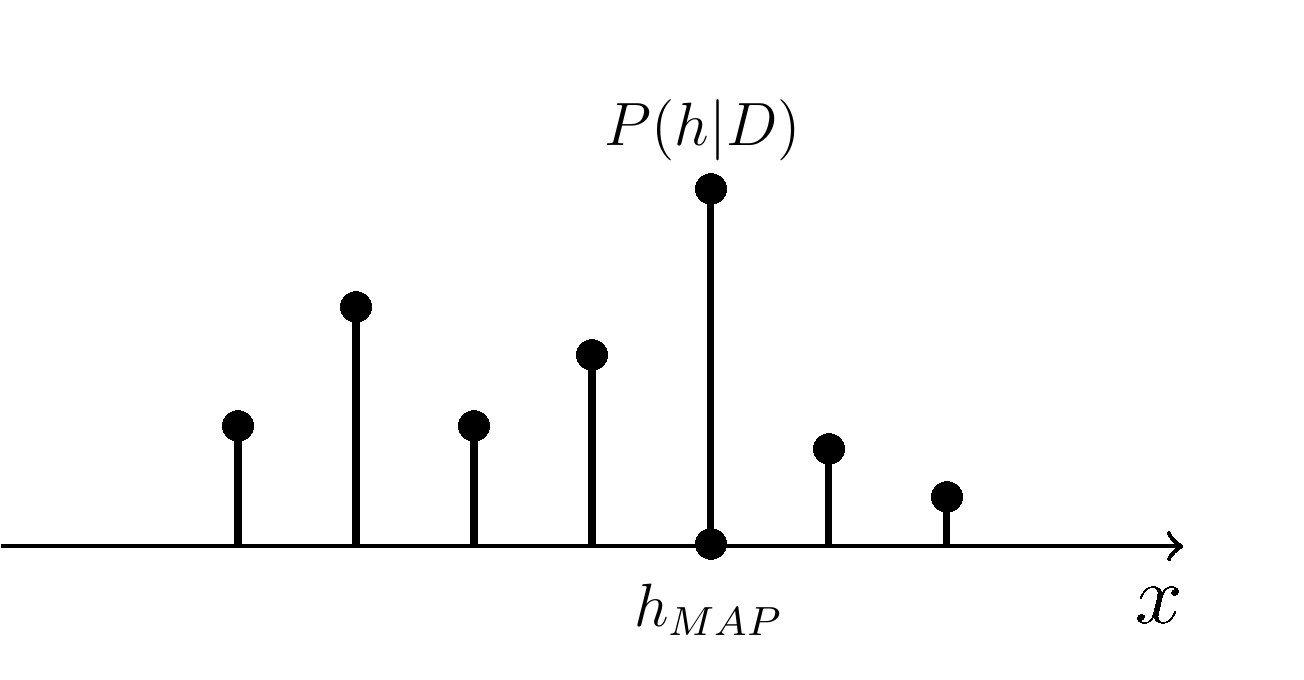
\includegraphics[width=.8\linewidth]{./images/discr}
		\caption{Discreto}
		\label{fig:discr}
	\end{subfigure}
	\begin{subfigure}{.5\textwidth}
		\centering
		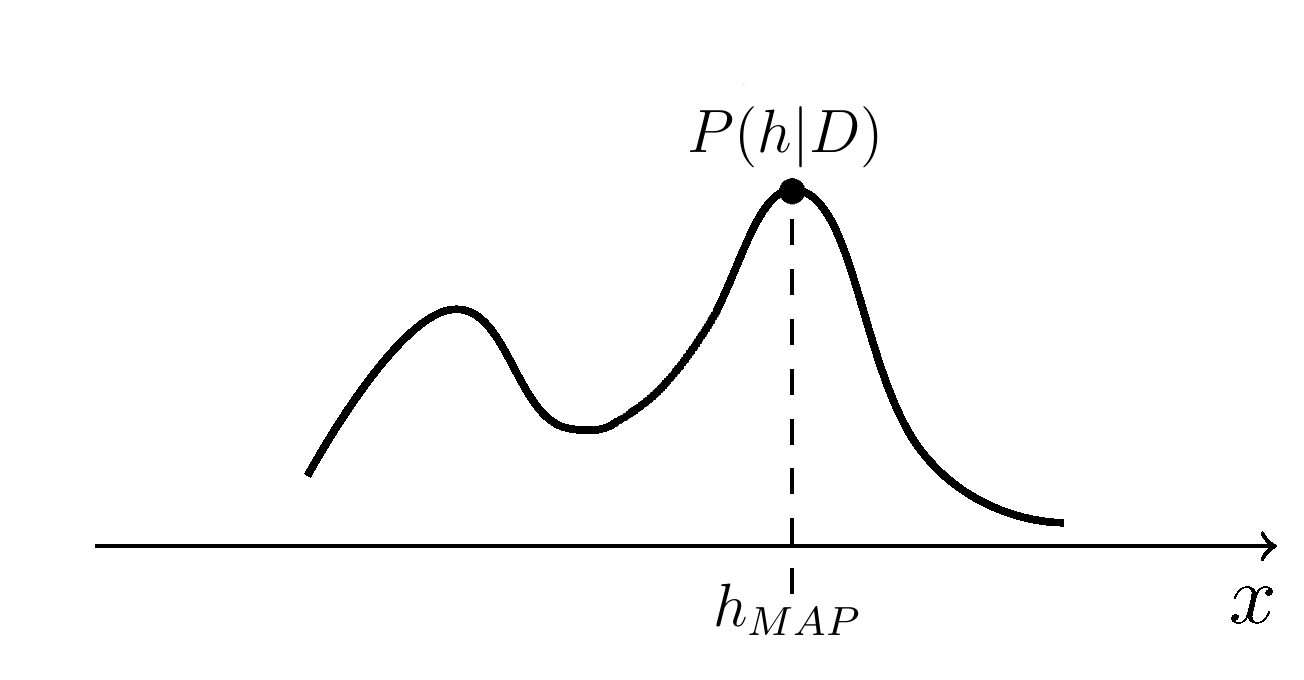
\includegraphics[width=.8\linewidth]{./images/cont}
		\caption{Continuo}
		\label{fig:cont}
	\end{subfigure}
	\caption{Rappresentazione di MAP}
	\label{fig:hmap}
\end{figure}

\section{Naive Bayes Classifier}
Un metodo di apprendimento molto efficace è il classificatore \emph{naive Bayes}. Esso si applica a task di apprendimento in cui ogni istanza è descritta come una congiunzione di valori di attributo $\langle a_1, ..., a_n \rangle$ e dove l'attributo target può assumere qualsiasi valore da un insieme finito $V$.

Ad una nuova istanza viene assegnato il più probabile valore target $v_{MAP}$, considerati i valori di attributo $\langle a_1, ..., a_n \rangle$:

$$ v_{MAP} = \argmax_{v_j \in V} P(v_j | a_1, ..., a_n) $$

Riapplicando le trasformazioni relative alla MAP definite sopra, possiamo riscrivere l'espressione come:

$$v_{MAP} = \argmax_{h \in H} \frac{P(a_1, ..., a_n | v_j) P(v_j)}{P(a_1, ..., a_n)} $$
$$\hphantom{11111} = \argmax_{h \in H} P(a_1, ..., a_n | v_j) P(v_j) $$

Ora bisogna stimare le due probabilità sui dati di training. I vari $P(v_j)$ possono essere facilmente calcolati contando la frequenza con cui ogni valore target $v_j$ occorre nei dati. Non è altrettanto semplice calcolare $P(a_1, ..., a_n | v_j)$ allo stesso modo. Il problema è che ci sono molte probabilità da calcolare e pochi dati a disposizione per ottenere delle stime affidabili: servirebbero dataset molto grandi.

Qui entra in gioco il punto cardine del NBC, ossia presupporre che esista l'\emph{indipendenza condizionale} tra gli attributi. In altre parole, l'assunzione è che, dato il valore target, la probabilità di osservare la congiunzione $a_1, ..., a_n$ è semplicemente il prodotto delle probabilità dei singoli attributi:

$$ P(a_1, ..., a_n | v_j) = \prod_i P(a_i|v_j) $$

\noindent
Facendo le opportune sostituzioni otteniamo:

$$ v_{NB} = v_{MAP} = \argmax_{v_j \in V} P(v_j) \prod_i P(a_i|v_j) $$

dove $v_{NB}$ è il valore target restituito da NBC, che è uguale a $v_{MAP}$ quando si assume l'indipendenza condizionale. Si noti che $P(a_i|v_j)$ è semplicemente il numero dei valori di attributo distinti moltiplicato il numero dei valori target distinti, chiaramente un numero molto più piccolo e gestibile rispetto a $P(a_1, ..., a_n | v_j)$ senza l'ipotesi di indipendenza. 

L'algoritmo di un NBC è pertanto:
\begin{itemize}
	\item Calcola i vari $P(v_j)$ e $P(a_i|v_j)$, basandoti sulle loro frequenze sui dati di training.
	\item Usa queste stime per formare l'ipotesi.
	\item Ogniqualvolta l'assunzione di indipendenza condizionale è soddisfatta, la classificazione $v_{NB}$ è uguale alla classificazione MAP.
\end{itemize}

Un aspetto interessante è che NBC non effettua alcuna ricerca esplicita nello spazio delle ipotesi. Viene costruita l'ipotesi semplicemente contando le frequenze delle varie combinazioni dei dati all'interno del training set.

\subsection*{Attributi continui}
Contare le frequenze delle diverse combinazioni di valori è possibile per gli attributi discreti, quindi bisogna trovare un modo per calcolare le probabilità degli eventuali attributi continui. Ci sono due strade: la prima è appunto discretizzare i valori numerici in vari \emph{bin}, l'altra è assumere l'esistenza di una distribuzione normale (Gaussiana) per i valori $\langle a_1, ..., a_n \rangle$ dell'attributo $A_k$. Questa funzione ha bisogno di due parametri, media e deviazione standard degli attributi:

$$ \mu_{kj} = E[A_k | v_j] = \frac{1}{n} \sum_{i = 1}^{n} a_i$$
$$ \sigma_{kj} = \sqrt{ E[(A_k - \mu_{kj})^2 | v_j] } = \sqrt{ \frac{1}{n-1} \sum_{i = 1}^{n} (a_i - \mu_{kj})^2 } $$

Infine, serve la funzione di densità di probabilità della Gaussiana, che applicata al nostro contesto diventa:

$$ P(a_i | v_j) = \frac{1}{\sqrt{2\pi} \sigma} e^{-\frac{(a_i-\mu)^2}{2\sigma^2}} $$

	\clearpage
	\chapter{REPTree}
\label{(ch:reptree)}

Come primo algoritmo si è scelto di usare \textbf{REPTree}, che costruisce alberi di decisione usando l'\textit{information gain} per i valori nominali e la varianza per i valori numerici\cite{2Witten:2011:DMP:REPTree}.

Visto che sono stati presi in considerazione dataset con attributi di classe nominali per un task di classificazione e non di regressione, verrà discusso il criterio dell'information gain, analogo all'algoritmo \textit{C4.5}\cite{Quinlan:1993:CPM:152181}.

\section{Information Gain}
Per selezionare l'attributo che meglio classifica i dati $D$ ed in particolare, su quale dei suoi valori occorre fare uno \textit{split}, può convenire usare l'\emph{entropia}\cite{Shannon:1948}, ossia l'incertezza contenuta nei dati, che è calcolata come:

$$ E(D) = - \sum_{i} p_i \log_2 p_i $$

cioè la media dei logaritmi delle probabilità di ciascun oggetto $i$ pesato per la probabilità stessa. Nel contesto di classificazione, gli oggetti sono gli esempi nel dataset di cui viene calcolata la probabilità che essi appartengano o meno ad una delle classi presenti nell'attributo target. Più è probabile che un esempio appartenga ad una certa classe, più la sua influenza nel calcolo della media sarà mitigata dal logaritmo della sua stessa probabilità.

È possibile calcolare l'entropia anche per sottoinsiemi del dataset, in particolare quegli esempi $D_v$ che presentano lo stesso valore $v$ di un certo attributo $a$, poi sommare tutte le entropie relative a tutti valori $V$ dell'attributo per ottenere l'entropia dei dati dopo aver preso in considerazione l'attributo $a$.
Ogni entropia viene pesata per il numero di esempi che presentano quel valore diviso per il totale di esempi esistenti nel dataset:

$$ E(D|a) = \sum_{v \in V} \frac{|D_v|}{|D|} \cdot E(D_v) $$

Da queste formule si ricava l'information gain, cioè la riduzione di incertezza totale prendendo in considerazione un attributo $a$:

$$ IG = E(D) - E(D|a) $$

Come radice verrà utilizzato l'attributo che massimizza l'information gain, come archi i valori dell'attributo e si ripete la procedura per i nodi figli fino a generare le foglie.

\section{Reduced Error Pruning}
\label{ss:rep}
Per evitare l'\textit{overfitting}, ossia un sovra-adattamento del modello ai dati di training che compromette la bontà delle sue predizioni su nuovi esempi, può essere ragionevole semplificare il modello, rischiando di commettere qualche errore ma garantendoci una migliore copertura per dati non visti.

Questa semplificazione viene chiamata \textit{pruning} (potatura), in cui, una volta costruito il modello utilizzando i dati del \textit{growing set}, esso viene testato su una parte dei dati, accantonati e non adoperati per la predizione, che fanno parte del \textit{pruning set}.

Una tecnica di potatura è REP (\textbf{R}educed \textbf{E}rror \textbf{P}runing)\cite{Quinlan:1987:SDT:50007.50008} che utilizza un pruning set per stimare l'accuratezza dei nodi intermedi e confrontarla con quella dei suoi sottoalberi.

Viene calcolato il guadagno dall'eventuale potatura sottraendo il numero di errori (esempi classificati scorrettamente) al sottoalbero $T$ al numero di errori al nodo radice $v$ del sottoalbero:

$$ Gain_{REP} = \varepsilon_T - \varepsilon_v $$

L'albero è potato se il guadagno è positivo quando vengono commessi più errori nell'intero sottoalbero, e non al nodo. C'è un'altra condizione da rispettare per procedere alla potatura: può avvenire solo se il sottoalbero $T$ non ha un sottoalbero che ha un tasso d'errore minore di $T$ stesso (\textit{bottom-up restriction}).

L'algoritmo di REP è il seguente:
\begin{itemize}
	\item Si parte dall'albero completo e lo si visita in post-ordine.
	\item Per ogni nodo intermedio $v$
	\begin{itemize}
		\item Calcolo l'accuratezza sul pruning set dell'albero completo.
		\item Calcolo l'accuratezza sul pruning set rispetto a $v$ e al suo sottoalbero $T$.
	\end{itemize}
	\item Se l'accuratezza aumenta, pota. In caso di uguaglianza pota per semplificare (rasoio di Occam).
\end{itemize}

Inoltre è dimostrato che, tra tutti i possibili sottoalberi potati che è possibile generare, REP trova il sottalbero più piccolo e più accurato rispetto al pruning set\cite{Esposito:1997:CAM:252862.252878}.
	\clearpage
	\chapter{RIPPER}
\label{ch:jrip}

Come ultimo algoritmo si è scelto di usare \textbf{RIPPER}\cite{Cohen95fasteffective}, in particolare nella versione implementata da Weka, \textbf{JRip}\cite{Witten:2011:DMP:1972514}.

RIPPER (\textbf{R}epeated \textbf{I}ncremental \textbf{P}runing to \textbf{P}roduce \textbf{E}rror \textbf{R}eduction) è un algoritmo di induzione di regole proposto da \verb|William W. Cohen| nel 1995. Esso si è dimostrato competitivo con C4.5Rules rispetto ai tassi di errore, scala in maniera lineare con il numero di esempi di training e può elaborare in maniera efficiente dataset rumorosi che contengono centinaia di migliaia di esempi. RIPPER si basa su IREP (\textbf{I}ncremental \textbf{R}educed \textbf{E}rror \textbf{P}runing))\cite{Furnkranz94incrementalreduced}, di cui si discuterà nei prossimi paragrafi.

Molte delle tecniche usate nei moderni sistemi di apprendimento di regole  sono stati adattate dall'apprendimento degli alberi di decisione. La maggior parte dei sistemi di apprendimento di alberi di decisione usa una strategia di appredimento \textit{overfit-and-simplify} (sovradatta-e-semplifica) per gestire dati rumorosi: viene generata un'ipotesi prima facendo crescere un albero complesso che "overfitta" i dati, e poi si semplifica o pota tale albero (un'operazione di \textit{pruning}). Una tecnica di pruning efficace è \textit{reduced error pruning} (\textit{REP}), discussa in \ref{ss:rep}. Essa può essere facilmente adattata ai sistemi di apprendimento di regole\cite{Pagallo1990}\cite{Brunk91aninvestigation}.

In REP per le regole, il training set viene diviso in \textit{growing set} e \textit{pruning set}. All'inizio, viene creato un \textit{rule set} di partenza che overfitta il growing set, usando qualche metodo euristico. Questo rule set spropositato viene poi semplificato ripetutamente applicando qualche operatore di pruning. Ad ogni fase di semplificatione, l'operatore di pruning scelto è quello che produce la più grande riduzione di errore sul pruning set. La semplificazione finisce quando il tasso di errore non si riduce ulteriormente applicando gli operatori di pruning.

REP per le regole di solito migliora davvero la perfomance di generalizzazione sui dati rumorosi\cite{Pagallo1990}\cite{Brunk91aninvestigation}\cite{Weiss91reducedcomplexity}\cite{Furnkranz94incrementalreduced}; tuttavia è computazionalmente costoso per grandi dataset\cite{Cohen93efficientpruning}.

In risposta all'inefficienza di REP, Fürnkranz e Widmer [1994] proposero un algoritmo di apprendimento chiamato \textit{incremental reduced error pruning} (\textit{IREP})\cite{Furnkranz94incrementalreduced}.

\section{Incremental Reduced Error Pruning}
L'idea di usare un pruning set separato per la potatura è REP. La variante che pota una regola subito dopo averla "fatta crescere" si chiama \textit{incremental reduced error pruning} (IREP)\cite{2Witten:2011:DMP:1972514}. Quest'ultima integra saldamente REP con un algoritmo di apprendimento di regole \textit{separate-and-conquer}. L'algoritmo \ref{alg:irep} ne presenta una versione a due classi. Come ogni algoritmo separate-and-conquer standard, IREP costruisce un ruleset in maniera \textit{greedy}, una regola alla volta. Dopo averne trovata una, tutti gli esempi coperti da quella regola (sia positivi che negativi) sono cancellati. Questo processo si ripete finché non ci sono più esempi positivi, o finché la regola trovata da IREP non presenta un grande tasso di errore, cosa inaccettabile.

Per costruire una regola, IREP usa la seguente strategia. Prima, gli esempi non coperti sono partizionati a caso in due sottoinsiemi, un growing e un pruning set. Nell'implementazione di Cohen, il growing set contiene 2/3 degli esempi.

Poi, una regola viene "fatta crescere". L'implementazione di Cohen di $GrowRule$ è una versione proposizionale di FOIL (First Order Inductive Learner), dove i letterali non si servono di predicati ma di uguaglianze (per valori discreti) e confronti numerici (per valori continui)\cite{Russell:2003:AIM:773294}. Esso inizia con una congiunzione vuota di condizioni (la regola vuota) e considera di aggiungere a questa qualsiasi condizione nella forma $A_d=v$, $A_c \leq \theta$ oppure $A_c \geq \theta$ dove $A_d$ è un attributo discreto e $v$ è un valore che può assumere, mentre $A_c$ è un attributo continuo e $\theta$ è un valore soglia. $GrowRule$ aggiunge ripetutamente la condizione che massimizza un'euristica di \emph{information gain}, nello specifico quella di FOIL, finché la regola non copre più esempi negativi nel growing set.

Siano $R_0$ e $R_1$ due regole, la seconda ottenuta dall'aggiunta di una condizione nel corpo della prima. L'information gain viene così calcolato:

$$
Gain_{IREP}(R_0,R_1) = t \cdot \left(\log{\dfrac{p_1}{p_1 + n_1}} - \log{\dfrac{p_0}{p_0 + n_0}}\right)
$$

dove $t$ riguarda gli esempi positivi coperti da $R_0$ che soddisfano anche $R_1$ dopo aver aggiunto una condizione, $p_0$ (rispettivamente $p_1$) sono gli esempi positivi coperti da $R_0$ (rispettivamente $R_1$) e  $n_0$ (rispettivamente $n_1$) sono gli esempi negativi coperti da $R_0$ (rispettivamente $R_1$).

L'idea alla base è che l'informazione totale che si guadagna è dato dal numero di tuple che soddisfano la nuova condizione moltiplicato l'informazione guadagnata in merito a ciascuna\cite{Quinlan1990}.

Dopo aver espanso una regola, essa viene immediatamente potata. Per prunarla, l'implementazione di Cohen cancella qualsiasi sequenza finale di condizioni dalla regola e sceglie l'eliminazione che massimizza la funzione
\begin{equation}
	\label{eq:rulval}
	v(Rule, PrunePos, PruneNeg) \equiv \frac{p + (N - n)}{P + N}
\end{equation}

dove $P$ (rispettivamente $N$) è il numero totale di esempi in $PrunePos$ \linebreak ($PruneNeg$) e $p$ ($n$) è il numero di esempi in $PrunePos$ ($PruneNeg$) coperti da $Rule$. Questo processo è ripetuto finché nessun altra cancellazione migliora il valore di $v$.

L'algoritmo IREP descritto sopra è per i problemi di apprendimento a due classi. L'implementazione di Cohen gestisce classi multiple, come spiegato di seguito:
\begin{enumerate}
	\item Le classi vengono ordinate secondo la prevalenza, cioè l'ordine è $C_1,...,C_k$ dove $C_1$ è la classe di minoranza e $C_k$ è la classe di maggioranza.
	\item Viene trovata una regola che separi $C_1$ dal resto delle classi; questo viene fatto con una singola chiamata ad IREP dove $PosData$ contiene gli esempi di classe $C_1$ e $NegData$ contiene gli esempi di classi $C_2,C_3,...,C_k$.
	\item Tutte le istanze coperte dal ruleset appena addestrato sono rimosse dal dataset e IREP si appresta a separare $C_2$ dalle classi $C_3,...,C_k$.
	\item Si ripete finché rimane la sola classe $C_k$. Quest'ultima verrà usata come classe di default.
\end{enumerate}

L'implementazione di Cohen differisce da quella di Fürnkranz e Widmer sotto molti aspetti. Quando le regole vengono potate, la nuova implementazione permette di cancellare qualsiasi sequenza finale di condizioni, mentre l'implementazione di Fürnkranz e Widmer permette solo la cancellazione di una singola condizione finale. L'algoritmo rivisitato permette anche di fermare l'aggiunta di regole al ruleset quando la regola appresa ha un tasso di errore superiore al 50\%, mentre quello di Fürnkranz e Widmer la ferma quando l'accuratezza della regola è minore dell'accuratezza della regola vuota.

\begin{algorithm}[!htbp]
	\caption{IREP($Pos, Neg$)}
	\label{alg:irep}
	\begin{algorithmic}[1]
		\State $Ruleset \gets \emptyset$
		
		\While{Pos $\neq \emptyset$}
		\State dividi $(Pos, Neg)$ in $(GrowPos, GrowNeg)$ e $(PrunePos, PrunNeg)$
		\State $Rule \gets GrowRule(GrowPos, GrowNeg)$
		\State $Rule \gets PruneRule(Rule, PrunePos, PruneNeg)$
		
		\If{il tasso di errore su $(PrunePos, PrunNeg) > 50\%$}
		\State \Return $Ruleset$
		\Else
		%\State $Ruleset \gets Ruleset \cup \{Rule\}$
		\State aggiungi $Rule$ a $Ruleset$
		\State rimuovi gli esempi coperti da $Rule$ da $(Pos, Neg)$
		\EndIf
		\EndWhile
		
		\State \Return $Ruleset$
	\end{algorithmic}
\end{algorithm}

\pagebreak

\section{Miglioramenti ad IREP}
Sono state implementate tre modifiche ad IREP: una metrica alternativa per determinare il valore delle regole nella fase di potatura; una nuova euristica per dedidere quando fermare l'aggiunta di regole al ruleset; un successivo passaggio di "ottimizzazione" del ruleset per tentare di avvicinarsi di più al REP convenzionale (cioè, non incrementale).

\subsection*{Metrica per il valore delle regole}
Il fallimento occasionale di IREP a convergere al crescere del numero degli esempi può essere facilmente fatto risalire alla metrica usata per guidare la potatura (ossia la \eqref{eq:rulval}). Le scelte intraprese nella definizione di tale metrica non sono intuitive; per esempio (assumendo che $P$ e $N$ siano fissati) la metrica preferisce una regola $R_1$ che copre $p_1 = 2000$ esempi positivi e $n_1 = 1000$ esempi negativi rispetto ad una regola $R_2$ che copre $p_2 = 1000$ esempi positivi e $n_2 = 1$ esempio negativo; si noti comunque che $R_2$ è altamente predittiva, al contrario di $R_1$. Quindi si è deciso di sostituire la metrica di IREP con $$v^*(Rule, PrunePos, PruneNeg) \equiv \frac{p - n}{p + n}$$ che sembra avere un comportamento più intuitivo e soddisfacente.

\subsection*{Condizione di stop}
L'implementazione di IREP di Cohen si ferma in maniera greedy aggiungendo regole al ruleset quando l'ultima regola costruita ha un tasso d'errore maggiore del 50\% sui dati di pruning. Questa euristica, spesso, si ferma troppo presto con campioni di dimensioni moderate; questo è vero soprattutto quando si apprende un concetto con regole a bassa copertura (pochi esempi coperti).

La soluzione a questo problema è la seguente. Dopo l'aggiunta di ogni regola, viene calcolata la \textit{description-length} totale del ruleset e degli esempi. La nuova versione di IREP ferma l'aggiunta di regole quando questa description-length è maggiore di $d$ bit rispetto alla più piccola description-length ottenuta sinora, o quando non ci sono più esempi positivi. Nell'implementazione si è usato $d = 64$. Il ruleset viene poi semplificato esaminando ogni regola a turno (cominciando dall'ultima) e cancellando regole così da ridurre la description-length totale.

Il principio \emph{MDL} (Minimum Description Length) può essere meglio espresso immaginando un modello di comunicazione in cui un mittente trasmette ad un ricevente una descrizione che consiste in una teoria $T$ e i dati $D$ da cui essa è derivata\cite{Quinlan:1989:IDT:70758.70761}.

Il metodo usato per la codifica è lo stesso usato in \emph{C4.5rules}\cite{Quinlan95mdland}. Esso parte da un \emph{bias} in cui il numero di falsi positivi e falsi negativi sia lo stesso e si procede come segue: i messaggi da inviare si presentano con probabilità $p_j$, e servono $-\log(p_j)$ bit (in base 2) per costrurli: più un messaggio è frequente, meno bit saranno necessari per rappresentarlo. Si inviano i dati codificati, poi anziché inviare i messaggi di errore per tutti i dati, il mittente prima trasmette gli errori $e$ nei $C$ casi coperti dalla teoria e poi negli $U$ casi non coperti. Sotto l'assunzione che i falsi positivi $fp$ e i falsi negativi $fn$ siano bilanciati, la probabilità di errore nei casi coperti è $e/2C$ e questa probabilità è usata per codificare i messaggi di errore per i casi coperti. Una volta che i falsi positivi sono stati identificati, il destinatario può calcolare il vero numero dei falsi negativi come $e-fp$, quindi la probabilità di errore oer i casi non coperti è $fn/U$. Il costo totale quindi diventa:

\begin{align*}
	&\log(|D| + 1) \\
	&+ fp \times (-\log(\dfrac{e}{2C})) \\
	&+ (C - fp) \times (-\log(1 - \-\dfrac{e}{2C})) \\
	&+ fn \times (-\log(\dfrac{fn}{U})) \\
	&+ (U - fn) \times (-\log(1 - \dfrac{fn}{U})) \\	
\end{align*}


\subsection*{Ottimizzazione delle regole}
L'approccio ripetuto \textit{grow-and-simplify} usato in IREP può produrre risultati abbastanzi differenti dal REP convenzionale (non incrementale). Un modo per migliorarlo è elaborare a posteriori le regole prodotte da IREP così da avvicinarsi di più all'effetto del REP convenzionale. Per esempio, si potrebbe ri-potare ogni regola al fine di minimizzare l'errore del ruleset completo.

Il metodo sviluppato per ottimizzare un ruleset $R_1,R_2,...,R_k$ consiste del costruire due regole alternative per ogni $R_i$. La \textit{sostituta} di $R_i$ viene generata espandendo e poi potando $R_i$. La \textit{revisione} di $R_i$ viene generata in maniera analoga, tranne per il fatto che la revisione è espansa in modo greedy aggiungendo condizioni a $R_i$, piuttosto che alla regola vuota. Infine si sceglie tra le tre regole quale includere nella teoria. Questa decisione viene presa in base all'euristica MDL. L'implementazione di questo metodo in IREP avviene in questo modo:
\begin{enumerate}
	\item Viene usato IREP per ottenere un ruleset iniziale.
	\item Esso viene ottimizzato, come descritto sopra.
	\item Vengono aggiunte le regole in modo tale da coprire gli esempi positivi rimanenti.
\end{enumerate}

L'ottimizzazione può essere ripetuta più volte elaborando il ruleset ottenuto dalla passata precedente dell'algoritmo.

IREP, con l'aggiunta del passo di post-ottimizzazione, forma un nuovo algoritmo che è stato chiamato \textbf{RIPPER} (\textbf{R}epeated \textbf{I}ncremental \textbf{P}runing to \textbf{P}roduce \textbf{E}rror \textbf{R}eduction).

L'implementazione in Weka di RIPPER si chiama JRip.
	\clearpage
	\chapter{Esecuzione}
\label{ch:results}
Qui vengono confrontati i due algoritmi REPTree e RIPPER/JRip. Entrambi hanno sfruttato una \textit{10-fold cross validation}.

\section{Risultati su \texttt{German Credit}}

\normalsize L'esecuzione ha coinvolto 900 istanze di training e 100 istanze di testing ad ogni iterazione del CV.

\begin{mdframed}[frametitle=Esecuzione NaiveBayesSimple]
	\footnotesize\verbatiminput{results/nb/german_credit.nb}
\end{mdframed}

\LTXtable{1.4\linewidth}{results/nb/german_credit.nbc}


\begin{mdframed}[frametitle=Esecuzione REPTree]
	\footnotesize\verbatiminput{results/reptree/german_credit.reptree}
\end{mdframed}


\begin{sidewaysfigure}
	\thisfloatpagestyle{empty}
	\makebox[\textwidth]{
\includegraphics[width=1.4\textwidth, height=.4\textheight]{results/reptree/gc.pdf}}
	\caption{Modello di REPTree}
\end{sidewaysfigure}

\pagebreak

\begin{mdframed}[frametitle=Esecuzione JRip]
	\footnotesize\verbatiminput{results/jrip/german_credit.jrip}
\end{mdframed}


\noindent
\normalsize Regole:
\input{results/jrip/german_credit.list.rules}

\pagebreak

\section{Risultati su \texttt{Hepatitis}}

\normalsize L'esecuzione ha coinvolto 139 istanze di training e 16 istanze di testing ad ogni iterazione del CV.

\begin{mdframed}[frametitle=Esecuzione NaiveBayesSimple]
	\footnotesize\verbatiminput{results/nb/hepatitis.nb}
\end{mdframed}


\scriptsize\input{results/nb/hepatitis.nbc}

\begin{mdframed}[frametitle=Esecuzione REPTree]
	\footnotesize\verbatiminput{results/reptree/hepatitis.reptree}
\end{mdframed}


\begin{figure}[htb]
	\makebox[\textwidth]{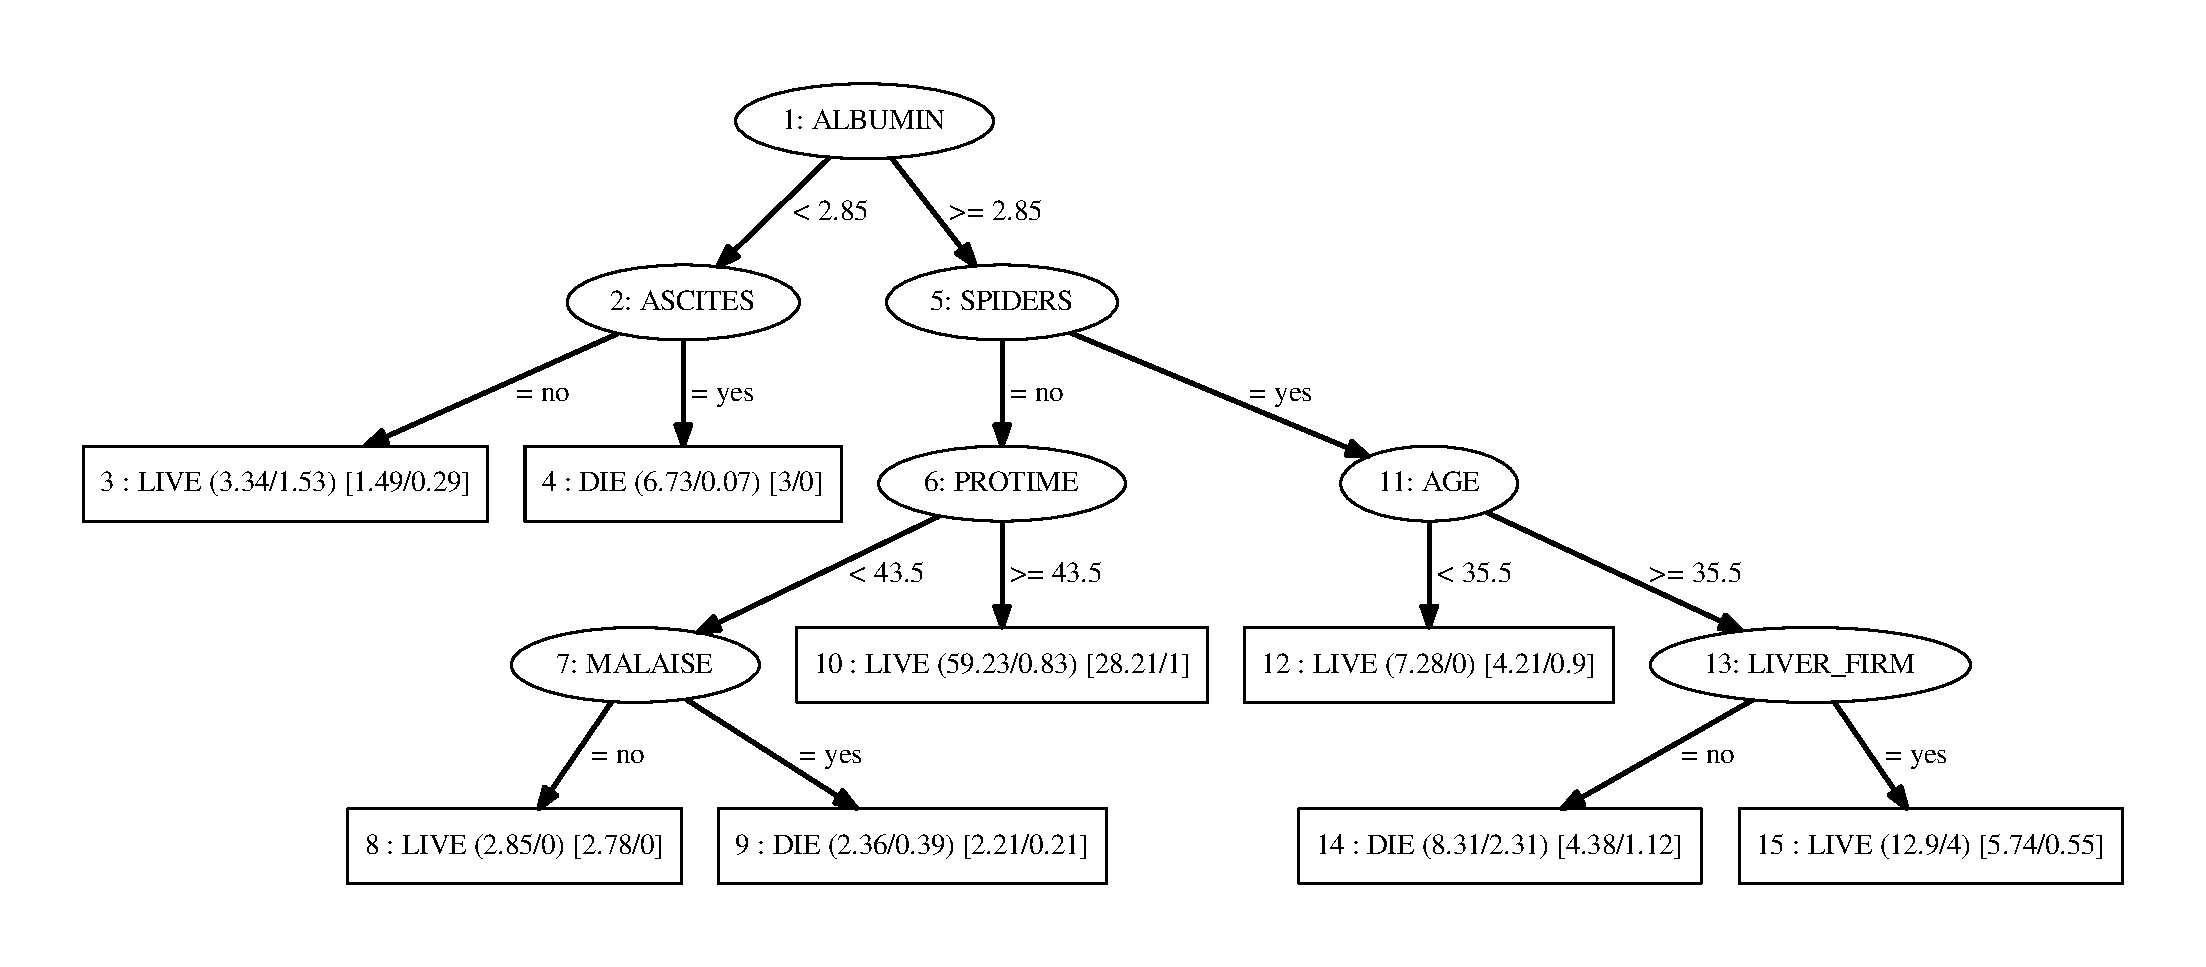
\includegraphics[width=1.55\textwidth]{results/reptree/hepatitis.pdf}}
	\caption{Modello di REPTree}
\end{figure}

\begin{mdframed}[frametitle=Esecuzione JRip]
	\footnotesize\verbatiminput{results/jrip/hepatitis.jrip}
\end{mdframed}


\noindent
\normalsize Regole:
\footnotesize\input{results/jrip/hepatitis.list.rules}

\pagebreak

\section{Risultati su \texttt{Vehicle Silhouettes}}

\normalsize L'esecuzione ha coinvolto 761 istanze di training e 85 istanze di testing ad ogni iterazione del CV.

\begin{mdframed}[frametitle=Esecuzione NaiveBayesSimple]
	\footnotesize\verbatiminput{results/nb/vehicle.nb}
\end{mdframed}


\scriptsize
\begin{tikzpicture}[>=latex,line join=bevel,]
  \pgfsetlinewidth{1bp}
%%
\pgfsetcolor{black}
  % Edge: N4cdf35a9 -> N4c98385c
  \draw [->,very thick] (855.15bp,368.07bp) .. controls (847.01bp,354.75bp) and (835.53bp,335.95bp)  .. (820.8bp,311.85bp);
  \definecolor{strokecol}{rgb}{0.0,0.0,0.0};
  \pgfsetstrokecolor{strokecol}
  \draw (863.5bp,340.0bp) node { < 127.5};
  % Edge: N442d9b6e -> N15615099
  \draw [->,very thick] (1228.1bp,368.7bp) .. controls (1247.8bp,354.57bp) and (1276.4bp,333.96bp)  .. (1306.8bp,312.1bp);
  \draw (1302.0bp,340.0bp) node { >= 62.5};
  % Edge: N20fa23c1 -> N3581c5f3
  \draw [->,very thick] (221.96bp,552.49bp) .. controls (204.16bp,538.19bp) and (178.26bp,517.38bp)  .. (150.54bp,495.1bp);
  \draw (215.0bp,524.0bp) node { < 67.5};
  % Edge: N2b05039f -> N61e717c2
  \draw [->,very thick] (457.14bp,276.49bp) .. controls (439.84bp,262.46bp) and (414.79bp,242.15bp)  .. (387.48bp,220.01bp);
  \draw (452.5bp,248.0bp) node { < 187.5};
  % Edge: N484b61fc -> N45fe3ee3
  \draw [->,very thick] (711.91bp,459.65bp) .. controls (707.74bp,446.7bp) and (701.96bp,428.76bp)  .. (694.07bp,404.3bp);
  \draw (724.0bp,432.0bp) node { < 17.5};
  % Edge: N1a93a7ca -> N3d82c5f3
  \draw [->,very thick] (370.43bp,368.2bp) .. controls (364.15bp,362.63bp) and (357.34bp,356.25bp)  .. (351.5bp,350.0bp) .. controls (342.86bp,340.75bp) and (334.11bp,329.9bp)  .. (320.75bp,312.23bp);
  \draw (365.5bp,340.0bp) node { < 99};
  % Edge: N58d25a40 -> N1b701da1
  \draw [->,very thick] (1058.6bp,551.65bp) .. controls (1057.1bp,538.82bp) and (1055.2bp,521.11bp)  .. (1052.4bp,496.3bp);
  \draw (1074.0bp,524.0bp) node { < 76.5};
  % Edge: N4cdf35a9 -> N73a8dfcc
  \draw [->,very thick] (887.98bp,368.28bp) .. controls (907.16bp,354.01bp) and (934.93bp,333.36bp)  .. (964.14bp,311.63bp);
  \draw (962.5bp,340.0bp) node { >= 127.5};
  % Edge: N4dcbadb4 -> N17d10166
  \draw [->,very thick] (368.85bp,92.072bp) .. controls (379.5bp,78.581bp) and (394.56bp,59.486bp)  .. (412.96bp,36.158bp);
  \draw (420.0bp,64.0bp) node { >= 66.5};
  % Edge: N504bae78 -> N368102c8
  \draw [->,very thick] (883.38bp,736.7bp) .. controls (909.86bp,722.26bp) and (948.75bp,701.04bp)  .. (987.16bp,680.1bp);
  \draw (971.5bp,708.0bp) node { >= 8.5};
  % Edge: N3b764bce -> N759ebb3d
  \draw [->,very thick] (853.5bp,643.65bp) .. controls (853.5bp,630.82bp) and (853.5bp,613.11bp)  .. (853.5bp,588.3bp);
  \draw (873.5bp,616.0bp) node { < 298.5};
  % Edge: N73a8dfcc -> N7e774085
  \draw [->,very thick] (1008.2bp,276.28bp) .. controls (1026.9bp,261.9bp) and (1054.1bp,241.02bp)  .. (1082.7bp,219.02bp);
  \draw (1076.5bp,248.0bp) node { >= 136};
  % Edge: N3b764bce -> N58d25a40
  \draw [->,very thick] (889.08bp,645.53bp) .. controls (924.14bp,630.29bp) and (977.82bp,606.95bp)  .. (1025.0bp,586.42bp);
  \draw (1001.5bp,616.0bp) node { >= 298.5};
  % Edge: N593634ad -> N20fa23c1
  \draw [->,very thick] (369.89bp,645.94bp) .. controls (344.87bp,631.22bp) and (306.55bp,608.67bp)  .. (269.74bp,587.02bp);
  \draw (351.0bp,616.0bp) node { < 95.5};
  % Edge: N7506e922 -> N504bae78
  \draw [->,very thick] (780.82bp,828.49bp) .. controls (794.45bp,814.71bp) and (814.07bp,794.87bp)  .. (836.67bp,772.01bp);
  \draw (840.0bp,800.0bp) node { >= 41.5};
  % Edge: N20fa23c1 -> N73c6c3b2
  \draw [->,very thick] (246.16bp,551.65bp) .. controls (248.87bp,538.82bp) and (252.61bp,521.11bp)  .. (257.85bp,496.3bp);
  \draw (277.0bp,524.0bp) node { >= 67.5};
  % Edge: N7e0b37bc -> N6ae40994
  \draw [->,very thick] (536.39bp,551.65bp) .. controls (538.54bp,538.74bp) and (541.52bp,520.88bp)  .. (545.67bp,495.99bp);
  \draw (567.5bp,524.0bp) node { >= 195.5};
  % Edge: N593634ad -> N48533e64
  \draw [->,very thick] (395.5bp,643.65bp) .. controls (395.5bp,630.82bp) and (395.5bp,613.11bp)  .. (395.5bp,588.3bp);
  \draw (418.0bp,616.0bp) node { >= 95.5};
  % Edge: N73a8dfcc -> Nea30797
  \draw [->,very thick] (984.19bp,275.65bp) .. controls (982.48bp,262.82bp) and (980.11bp,245.11bp)  .. (976.81bp,220.3bp);
  \draw (999.0bp,248.0bp) node { < 136};
  % Edge: N442d9b6e -> Nee7d9f1
  \draw [->,very thick] (1204.5bp,367.65bp) .. controls (1203.8bp,354.82bp) and (1202.8bp,337.11bp)  .. (1201.5bp,312.3bp);
  \draw (1221.0bp,340.0bp) node { < 62.5};
  % Edge: N5fcfe4b2 -> N5eb5c224
  \draw [->,very thick] (696.13bp,184.49bp) .. controls (712.73bp,170.52bp) and (736.74bp,150.33bp)  .. (763.27bp,128.01bp);
  \draw (763.0bp,156.0bp) node { >= 68.5};
  % Edge: N2b05039f -> N66cd51c3
  \draw [->,very thick] (483.09bp,275.65bp) .. controls (487.29bp,262.62bp) and (493.12bp,244.53bp)  .. (501.02bp,219.99bp);
  \draw (520.5bp,248.0bp) node { >= 187.5};
  % Edge: N7e774085 -> N3f8f9dd6
  \draw [->,very thick] (1091.1bp,184.07bp) .. controls (1081.3bp,170.71bp) and (1067.4bp,151.84bp)  .. (1050.1bp,128.16bp);
  \draw (1094.0bp,156.0bp) node { < 37.5};
  % Edge: N66cd51c3 -> N1b9e1916
  \draw [->,very thick] (508.62bp,183.65bp) .. controls (510.19bp,170.82bp) and (512.35bp,153.11bp)  .. (515.39bp,128.3bp);
  \draw (538.5bp,156.0bp) node { >= 204.5};
  % Edge: N64a294a6 -> N4f8e5cde
  \draw [->,very thick] (603.49bp,644.07bp) .. controls (616.35bp,630.46bp) and (634.6bp,611.13bp)  .. (656.29bp,588.16bp);
  \draw (659.5bp,616.0bp) node { >= 721};
  % Edge: N4ee285c6 -> N593634ad
  \draw [->,very thick] (553.62bp,737.12bp) .. controls (520.55bp,721.62bp) and (470.26bp,698.04bp)  .. (425.88bp,677.24bp);
  \draw (524.5bp,708.0bp) node { < 7.5};
  % Edge: N484b61fc -> N4cdf35a9
  \draw [->,very thick] (744.3bp,460.7bp) .. controls (768.25bp,446.14bp) and (803.52bp,424.69bp)  .. (838.4bp,403.48bp);
  \draw (828.0bp,432.0bp) node { >= 17.5};
  % Edge: N3581c5f3 -> N6aa8ceb6
  \draw [->,very thick] (116.38bp,460.49bp) .. controls (104.69bp,446.84bp) and (87.923bp,427.23bp)  .. (68.057bp,404.01bp);
  \draw (119.5bp,432.0bp) node { < 161.5};
  % Edge: N7e774085 -> Naec6354
  \draw [->,very thick] (1115.9bp,184.07bp) .. controls (1125.7bp,170.71bp) and (1139.6bp,151.84bp)  .. (1156.9bp,128.16bp);
  \draw (1165.0bp,156.0bp) node { >= 37.5};
  % Edge: N58d25a40 -> N1edf1c96
  \draw [->,very thick] (1088.4bp,552.91bp) .. controls (1113.5bp,538.45bp) and (1150.5bp,517.08bp)  .. (1187.0bp,496.02bp);
  \draw (1175.0bp,524.0bp) node { >= 76.5};
  % Edge: N3581c5f3 -> N2530c12
  \draw [->,very thick] (139.9bp,460.07bp) .. controls (147.26bp,446.83bp) and (157.62bp,428.19bp)  .. (170.97bp,404.16bp);
  \draw (185.5bp,432.0bp) node { >= 161.5};
  % Edge: N64a294a6 -> N7e0b37bc
  \draw [->,very thick] (577.34bp,644.07bp) .. controls (569.35bp,630.75bp) and (558.07bp,611.95bp)  .. (543.61bp,587.85bp);
  \draw (582.0bp,616.0bp) node { < 721};
  % Edge: N4c98385c -> N53e25b76
  \draw [->,very thick] (814.93bp,275.65bp) .. controls (818.21bp,262.82bp) and (822.74bp,245.11bp)  .. (829.08bp,220.3bp);
  \draw (847.0bp,248.0bp) node { >= 88.5};
  % Edge: N759ebb3d -> N484b61fc
  \draw [->,very thick] (828.56bp,552.49bp) .. controls (806.7bp,538.03bp) and (774.77bp,516.9bp)  .. (742.29bp,495.4bp);
  \draw (818.5bp,524.0bp) node { < 131.5};
  % Edge: N5fcfe4b2 -> N6bf2d08e
  \draw [->,very thick] (672.45bp,183.65bp) .. controls (669.46bp,170.82bp) and (665.33bp,153.11bp)  .. (659.54bp,128.3bp);
  \draw (686.0bp,156.0bp) node { < 68.5};
  % Edge: N504bae78 -> N3b764bce
  \draw [->,very thick] (853.5bp,735.65bp) .. controls (853.5bp,722.82bp) and (853.5bp,705.11bp)  .. (853.5bp,680.3bp);
  \draw (868.5bp,708.0bp) node { < 8.5};
  % Edge: N4ee285c6 -> N64a294a6
  \draw [->,very thick] (587.5bp,735.65bp) .. controls (587.5bp,722.82bp) and (587.5bp,705.11bp)  .. (587.5bp,680.3bp);
  \draw (607.5bp,708.0bp) node { >= 7.5};
  % Edge: N6ae40994 -> N1a93a7ca
  \draw [->,very thick] (522.05bp,461.94bp) .. controls (496.21bp,447.22bp) and (456.64bp,424.67bp)  .. (418.63bp,403.02bp);
  \draw (504.5bp,432.0bp) node { < 109.5};
  % Edge: N1b701da1 -> N726f3b58
  \draw [->,very thick] (1049.5bp,459.65bp) .. controls (1048.8bp,446.82bp) and (1047.8bp,429.11bp)  .. (1046.5bp,404.3bp);
  \draw (1066.0bp,432.0bp) node { < 10.5};
  % Edge: N4c98385c -> N5fcfe4b2
  \draw [->,very thick] (787.16bp,277.32bp) .. controls (765.65bp,262.88bp) and (733.52bp,241.3bp)  .. (700.93bp,219.41bp);
  \draw (774.0bp,248.0bp) node { < 88.5};
  % Edge: N4dcbadb4 -> N4e515669
  \draw [->,very thick] (342.15bp,92.072bp) .. controls (331.5bp,78.581bp) and (316.44bp,59.486bp)  .. (298.04bp,36.158bp);
  \draw (344.0bp,64.0bp) node { < 66.5};
  % Edge: N759ebb3d -> N1c655221
  \draw [->,very thick] (859.67bp,551.65bp) .. controls (864.27bp,538.7bp) and (870.65bp,520.76bp)  .. (879.35bp,496.3bp);
  \draw (897.5bp,524.0bp) node { >= 131.5};
  % Edge: N6ae40994 -> Nba8a1dc
  \draw [->,very thick] (548.89bp,459.65bp) .. controls (549.17bp,446.82bp) and (549.56bp,429.11bp)  .. (550.12bp,404.3bp);
  \draw (575.5bp,432.0bp) node { >= 109.5};
  % Edge: N66cd51c3 -> N4dcbadb4
  \draw [->,very thick] (480.54bp,185.53bp) .. controls (456.0bp,170.9bp) and (418.94bp,148.81bp)  .. (382.65bp,127.18bp);
  \draw (465.5bp,156.0bp) node { < 204.5};
  % Edge: N1b701da1 -> N442d9b6e
  \draw [->,very thick] (1078.2bp,460.91bp) .. controls (1103.7bp,446.13bp) and (1141.6bp,424.13bp)  .. (1178.0bp,402.95bp);
  \draw (1165.0bp,432.0bp) node { >= 10.5};
  % Edge: N7e0b37bc -> N3b95a09c
  \draw [->,very thick] (511.69bp,552.91bp) .. controls (492.57bp,538.8bp) and (464.54bp,518.13bp)  .. (434.78bp,496.18bp);
  \draw (503.5bp,524.0bp) node { < 195.5};
  % Edge: N7506e922 -> N4ee285c6
  \draw [->,very thick] (734.87bp,829.94bp) .. controls (705.67bp,815.09bp) and (660.82bp,792.28bp)  .. (619.01bp,771.02bp);
  \draw (710.0bp,800.0bp) node { < 41.5};
  % Edge: N1a93a7ca -> N2b05039f
  \draw [->,very thick] (406.86bp,368.07bp) .. controls (420.23bp,354.24bp) and (439.29bp,334.53bp)  .. (461.21bp,311.85bp);
  \draw (461.0bp,340.0bp) node { >= 99};
  % Node: N2b05039f
\begin{scope}
  \definecolor{strokecol}{rgb}{0.0,0.0,0.0};
  \pgfsetstrokecolor{strokecol}
  \draw (477.5bp,294.0bp) node {16: KURTOSIS ABOUT\_MINOR};
\end{scope}
  % Node: N1b701da1
\begin{scope}
  \definecolor{strokecol}{rgb}{0.0,0.0,0.0};
  \pgfsetstrokecolor{strokecol}
  \draw (1050.5bp,478.0bp) node {43: SKEWNESS ABOUT\_MINOR};
\end{scope}
  % Node: N4e515669
\begin{scope}
  \definecolor{strokecol}{rgb}{0.0,0.0,0.0};
  \pgfsetstrokecolor{strokecol}
  \draw (284.5bp,18.0bp) node {20 : opel (13/2) [2/0]};
\end{scope}
  % Node: N17d10166
\begin{scope}
  \definecolor{strokecol}{rgb}{0.0,0.0,0.0};
  \pgfsetstrokecolor{strokecol}
  \draw (426.5bp,18.0bp) node {21 : saab (36/11) [29/10]};
\end{scope}
  % Node: N6aa8ceb6
\begin{scope}
  \definecolor{strokecol}{rgb}{0.0,0.0,0.0};
  \pgfsetstrokecolor{strokecol}
  \draw (107.0bp,404.0bp) -- (0.0bp,404.0bp) -- (0.0bp,368.0bp) -- (107.0bp,368.0bp) -- cycle;
  \draw (53.5bp,386.0bp) node {6 : saab (4/0) [1/0]};
\end{scope}
  % Node: N1a93a7ca
\begin{scope}
  \definecolor{strokecol}{rgb}{0.0,0.0,0.0};
  \pgfsetstrokecolor{strokecol}
  \draw (390.5bp,386.0bp) node {14: DISTANCE CIRCULARITY};
\end{scope}
  % Node: N4ee285c6
\begin{scope}
  \definecolor{strokecol}{rgb}{0.0,0.0,0.0};
  \pgfsetstrokecolor{strokecol}
  \draw (587.5bp,754.0bp) node {2: MAX.LENGTH ASPECT RATIO};
\end{scope}
  % Node: N66cd51c3
\begin{scope}
  \definecolor{strokecol}{rgb}{0.0,0.0,0.0};
  \pgfsetstrokecolor{strokecol}
  \draw (506.5bp,202.0bp) node {18: HOLLOWS RATIO};
\end{scope}
  % Node: N5eb5c224
\begin{scope}
  \definecolor{strokecol}{rgb}{0.0,0.0,0.0};
  \pgfsetstrokecolor{strokecol}
  \draw (839.0bp,128.0bp) -- (728.0bp,128.0bp) -- (728.0bp,92.0bp) -- (839.0bp,92.0bp) -- cycle;
  \draw (783.5bp,110.0bp) node {34 : opel (2/0) [1/0]};
\end{scope}
  % Node: Nee7d9f1
\begin{scope}
  \definecolor{strokecol}{rgb}{0.0,0.0,0.0};
  \pgfsetstrokecolor{strokecol}
  \draw (1200.5bp,294.0bp) node {46 : opel (12/4) [5/2]};
\end{scope}
  % Node: N368102c8
\begin{scope}
  \definecolor{strokecol}{rgb}{0.0,0.0,0.0};
  \pgfsetstrokecolor{strokecol}
  \draw (1018.5bp,662.0bp) node {49 : van (73/4) [43/6]};
\end{scope}
  % Node: N1c655221
\begin{scope}
  \definecolor{strokecol}{rgb}{0.0,0.0,0.0};
  \pgfsetstrokecolor{strokecol}
  \draw (885.5bp,478.0bp) node {41 : van (54/8) [24/8]};
\end{scope}
  % Node: N7e0b37bc
\begin{scope}
  \definecolor{strokecol}{rgb}{0.0,0.0,0.0};
  \pgfsetstrokecolor{strokecol}
  \draw (533.5bp,570.0bp) node {11: HOLLOWS RATIO};
\end{scope}
  % Node: Naec6354
\begin{scope}
  \definecolor{strokecol}{rgb}{0.0,0.0,0.0};
  \pgfsetstrokecolor{strokecol}
  \draw (1225.0bp,128.0bp) -- (1114.0bp,128.0bp) -- (1114.0bp,92.0bp) -- (1225.0bp,92.0bp) -- cycle;
  \draw (1169.5bp,110.0bp) node {40 : opel (8/2) [1/0]};
\end{scope}
  % Node: N2530c12
\begin{scope}
  \definecolor{strokecol}{rgb}{0.0,0.0,0.0};
  \pgfsetstrokecolor{strokecol}
  \draw (236.0bp,404.0bp) -- (125.0bp,404.0bp) -- (125.0bp,368.0bp) -- (236.0bp,368.0bp) -- cycle;
  \draw (180.5bp,386.0bp) node {7 : opel (13/6) [3/1]};
\end{scope}
  % Node: N504bae78
\begin{scope}
  \definecolor{strokecol}{rgb}{0.0,0.0,0.0};
  \pgfsetstrokecolor{strokecol}
  \draw (853.5bp,754.0bp) node {25: MAX.LENGTH ASPECT RATIO};
\end{scope}
  % Node: N484b61fc
\begin{scope}
  \definecolor{strokecol}{rgb}{0.0,0.0,0.0};
  \pgfsetstrokecolor{strokecol}
  \draw (717.5bp,478.0bp) node {28: PR.AXIS RECTANGULARITY};
\end{scope}
  % Node: N1edf1c96
\begin{scope}
  \definecolor{strokecol}{rgb}{0.0,0.0,0.0};
  \pgfsetstrokecolor{strokecol}
  \draw (1277.0bp,496.0bp) -- (1156.0bp,496.0bp) -- (1156.0bp,460.0bp) -- (1277.0bp,460.0bp) -- cycle;
  \draw (1216.5bp,478.0bp) node {48 : opel (21/9) [13/8]};
\end{scope}
  % Node: N4c98385c
\begin{scope}
  \definecolor{strokecol}{rgb}{0.0,0.0,0.0};
  \pgfsetstrokecolor{strokecol}
  \draw (810.5bp,294.0bp) node {31: COMPACTNESS};
\end{scope}
  % Node: N45fe3ee3
\begin{scope}
  \definecolor{strokecol}{rgb}{0.0,0.0,0.0};
  \pgfsetstrokecolor{strokecol}
  \draw (688.5bp,386.0bp) node {29 : van (20/8) [10/4]};
\end{scope}
  % Node: N726f3b58
\begin{scope}
  \definecolor{strokecol}{rgb}{0.0,0.0,0.0};
  \pgfsetstrokecolor{strokecol}
  \draw (1107.0bp,404.0bp) -- (984.0bp,404.0bp) -- (984.0bp,368.0bp) -- (1107.0bp,368.0bp) -- cycle;
  \draw (1045.5bp,386.0bp) node {44 : bus (85/11) [58/9]};
\end{scope}
  % Node: N4cdf35a9
\begin{scope}
  \definecolor{strokecol}{rgb}{0.0,0.0,0.0};
  \pgfsetstrokecolor{strokecol}
  \draw (865.5bp,386.0bp) node {30: SCALED RADIUS OF GYRATION};
\end{scope}
  % Node: N5fcfe4b2
\begin{scope}
  \definecolor{strokecol}{rgb}{0.0,0.0,0.0};
  \pgfsetstrokecolor{strokecol}
  \draw (676.5bp,202.0bp) node {32: DISTANCE CIRCULARITY};
\end{scope}
  % Node: N15615099
\begin{scope}
  \definecolor{strokecol}{rgb}{0.0,0.0,0.0};
  \pgfsetstrokecolor{strokecol}
  \draw (1330.5bp,294.0bp) node {47 : bus (2/0) [1/0]};
\end{scope}
  % Node: N442d9b6e
\begin{scope}
  \definecolor{strokecol}{rgb}{0.0,0.0,0.0};
  \pgfsetstrokecolor{strokecol}
  \draw (1205.5bp,386.0bp) node {45: PR.AXIS ASPECT RATIO};
\end{scope}
  % Node: N6bf2d08e
\begin{scope}
  \definecolor{strokecol}{rgb}{0.0,0.0,0.0};
  \pgfsetstrokecolor{strokecol}
  \draw (655.5bp,110.0bp) node {33 : van (2/0) [1/0]};
\end{scope}
  % Node: N3b764bce
\begin{scope}
  \definecolor{strokecol}{rgb}{0.0,0.0,0.0};
  \pgfsetstrokecolor{strokecol}
  \draw (853.5bp,662.0bp) node {26: SCALED VARIANCE\_MINOR};
\end{scope}
  % Node: N64a294a6
\begin{scope}
  \definecolor{strokecol}{rgb}{0.0,0.0,0.0};
  \pgfsetstrokecolor{strokecol}
  \draw (587.5bp,662.0bp) node {10: SCALED VARIANCE\_MINOR};
\end{scope}
  % Node: N3581c5f3
\begin{scope}
  \definecolor{strokecol}{rgb}{0.0,0.0,0.0};
  \pgfsetstrokecolor{strokecol}
  \draw (130.5bp,478.0bp) node {5: SCATTER RATIO};
\end{scope}
  % Node: Nba8a1dc
\begin{scope}
  \definecolor{strokecol}{rgb}{0.0,0.0,0.0};
  \pgfsetstrokecolor{strokecol}
  \draw (609.0bp,404.0bp) -- (492.0bp,404.0bp) -- (492.0bp,368.0bp) -- (609.0bp,368.0bp) -- cycle;
  \draw (550.5bp,386.0bp) node {23 : saab (13/0) [3/0]};
\end{scope}
  % Node: N58d25a40
\begin{scope}
  \definecolor{strokecol}{rgb}{0.0,0.0,0.0};
  \pgfsetstrokecolor{strokecol}
  \draw (1060.5bp,570.0bp) node {42: DISTANCE CIRCULARITY};
\end{scope}
  % Node: N48533e64
\begin{scope}
  \definecolor{strokecol}{rgb}{0.0,0.0,0.0};
  \pgfsetstrokecolor{strokecol}
  \draw (452.0bp,588.0bp) -- (339.0bp,588.0bp) -- (339.0bp,552.0bp) -- (452.0bp,552.0bp) -- cycle;
  \draw (395.5bp,570.0bp) node {9 : bus (52/0) [18/1]};
\end{scope}
  % Node: N759ebb3d
\begin{scope}
  \definecolor{strokecol}{rgb}{0.0,0.0,0.0};
  \pgfsetstrokecolor{strokecol}
  \draw (853.5bp,570.0bp) node {27: MAX.LENGTH RECTANGULARITY};
\end{scope}
  % Node: N1b9e1916
\begin{scope}
  \definecolor{strokecol}{rgb}{0.0,0.0,0.0};
  \pgfsetstrokecolor{strokecol}
  \draw (517.5bp,110.0bp) node {22 : saab (8/0) [7/4]};
\end{scope}
  % Node: N4f8e5cde
\begin{scope}
  \definecolor{strokecol}{rgb}{0.0,0.0,0.0};
  \pgfsetstrokecolor{strokecol}
  \draw (672.5bp,570.0bp) node {24 : opel (16/1) [8/1]};
\end{scope}
  % Node: N20fa23c1
\begin{scope}
  \definecolor{strokecol}{rgb}{0.0,0.0,0.0};
  \pgfsetstrokecolor{strokecol}
  \draw (242.5bp,570.0bp) node {4: PR.AXIS ASPECT RATIO};
\end{scope}
  % Node: N73c6c3b2
\begin{scope}
  \definecolor{strokecol}{rgb}{0.0,0.0,0.0};
  \pgfsetstrokecolor{strokecol}
  \draw (261.5bp,478.0bp) node {8 : bus (13/0) [3/0]};
\end{scope}
  % Node: N73a8dfcc
\begin{scope}
  \definecolor{strokecol}{rgb}{0.0,0.0,0.0};
  \pgfsetstrokecolor{strokecol}
  \draw (986.5bp,294.0bp) node {36: SCALED RADIUS OF GYRATION};
\end{scope}
  % Node: N4dcbadb4
\begin{scope}
  \definecolor{strokecol}{rgb}{0.0,0.0,0.0};
  \pgfsetstrokecolor{strokecol}
  \draw (355.5bp,110.0bp) node {19: SKEWNESS ABOUT\_MAJOR};
\end{scope}
  % Node: N6ae40994
\begin{scope}
  \definecolor{strokecol}{rgb}{0.0,0.0,0.0};
  \pgfsetstrokecolor{strokecol}
  \draw (548.5bp,478.0bp) node {13: COMPACTNESS};
\end{scope}
  % Node: N3f8f9dd6
\begin{scope}
  \definecolor{strokecol}{rgb}{0.0,0.0,0.0};
  \pgfsetstrokecolor{strokecol}
  \draw (1096.0bp,128.0bp) -- (979.0bp,128.0bp) -- (979.0bp,92.0bp) -- (1096.0bp,92.0bp) -- cycle;
  \draw (1037.5bp,110.0bp) node {39 : saab (12/2) [2/0]};
\end{scope}
  % Node: N7e774085
\begin{scope}
  \definecolor{strokecol}{rgb}{0.0,0.0,0.0};
  \pgfsetstrokecolor{strokecol}
  \draw (1103.5bp,202.0bp) node {38: CIRCULARITY};
\end{scope}
  % Node: N61e717c2
\begin{scope}
  \definecolor{strokecol}{rgb}{0.0,0.0,0.0};
  \pgfsetstrokecolor{strokecol}
  \draw (425.0bp,220.0bp) -- (308.0bp,220.0bp) -- (308.0bp,184.0bp) -- (425.0bp,184.0bp) -- cycle;
  \draw (366.5bp,202.0bp) node {17 : saab (14/0) [5/2]};
\end{scope}
  % Node: N53e25b76
\begin{scope}
  \definecolor{strokecol}{rgb}{0.0,0.0,0.0};
  \pgfsetstrokecolor{strokecol}
  \draw (833.5bp,202.0bp) node {35 : saab (4/1) [2/2]};
\end{scope}
  % Node: N7506e922
\begin{scope}
  \definecolor{strokecol}{rgb}{0.0,0.0,0.0};
  \pgfsetstrokecolor{strokecol}
  \draw (764.5bp,846.0bp) node {1: ELONGATEDNESS};
\end{scope}
  % Node: N593634ad
\begin{scope}
  \definecolor{strokecol}{rgb}{0.0,0.0,0.0};
  \pgfsetstrokecolor{strokecol}
  \draw (395.5bp,662.0bp) node {3: COMPACTNESS};
\end{scope}
  % Node: N3b95a09c
\begin{scope}
  \definecolor{strokecol}{rgb}{0.0,0.0,0.0};
  \pgfsetstrokecolor{strokecol}
  \draw (472.0bp,496.0bp) -- (351.0bp,496.0bp) -- (351.0bp,460.0bp) -- (472.0bp,460.0bp) -- cycle;
  \draw (411.5bp,478.0bp) node {12 : opel (27/4) [12/3]};
\end{scope}
  % Node: Nea30797
\begin{scope}
  \definecolor{strokecol}{rgb}{0.0,0.0,0.0};
  \pgfsetstrokecolor{strokecol}
  \draw (1030.0bp,220.0bp) -- (919.0bp,220.0bp) -- (919.0bp,184.0bp) -- (1030.0bp,184.0bp) -- cycle;
  \draw (974.5bp,202.0bp) node {37 : opel (4/0) [4/2]};
\end{scope}
  % Node: N3d82c5f3
\begin{scope}
  \definecolor{strokecol}{rgb}{0.0,0.0,0.0};
  \pgfsetstrokecolor{strokecol}
  \draw (374.0bp,312.0bp) -- (243.0bp,312.0bp) -- (243.0bp,276.0bp) -- (374.0bp,276.0bp) -- cycle;
  \draw (308.5bp,294.0bp) node {15 : opel (56/26) [26/12]};
\end{scope}
%
\end{tikzpicture}



\begin{mdframed}[frametitle=Esecuzione REPTree]
	\scriptsize\verbatiminput{results/reptree/vehicle.reptree}
\end{mdframed}


\begin{figure}[htb]
	\makebox[\textwidth]{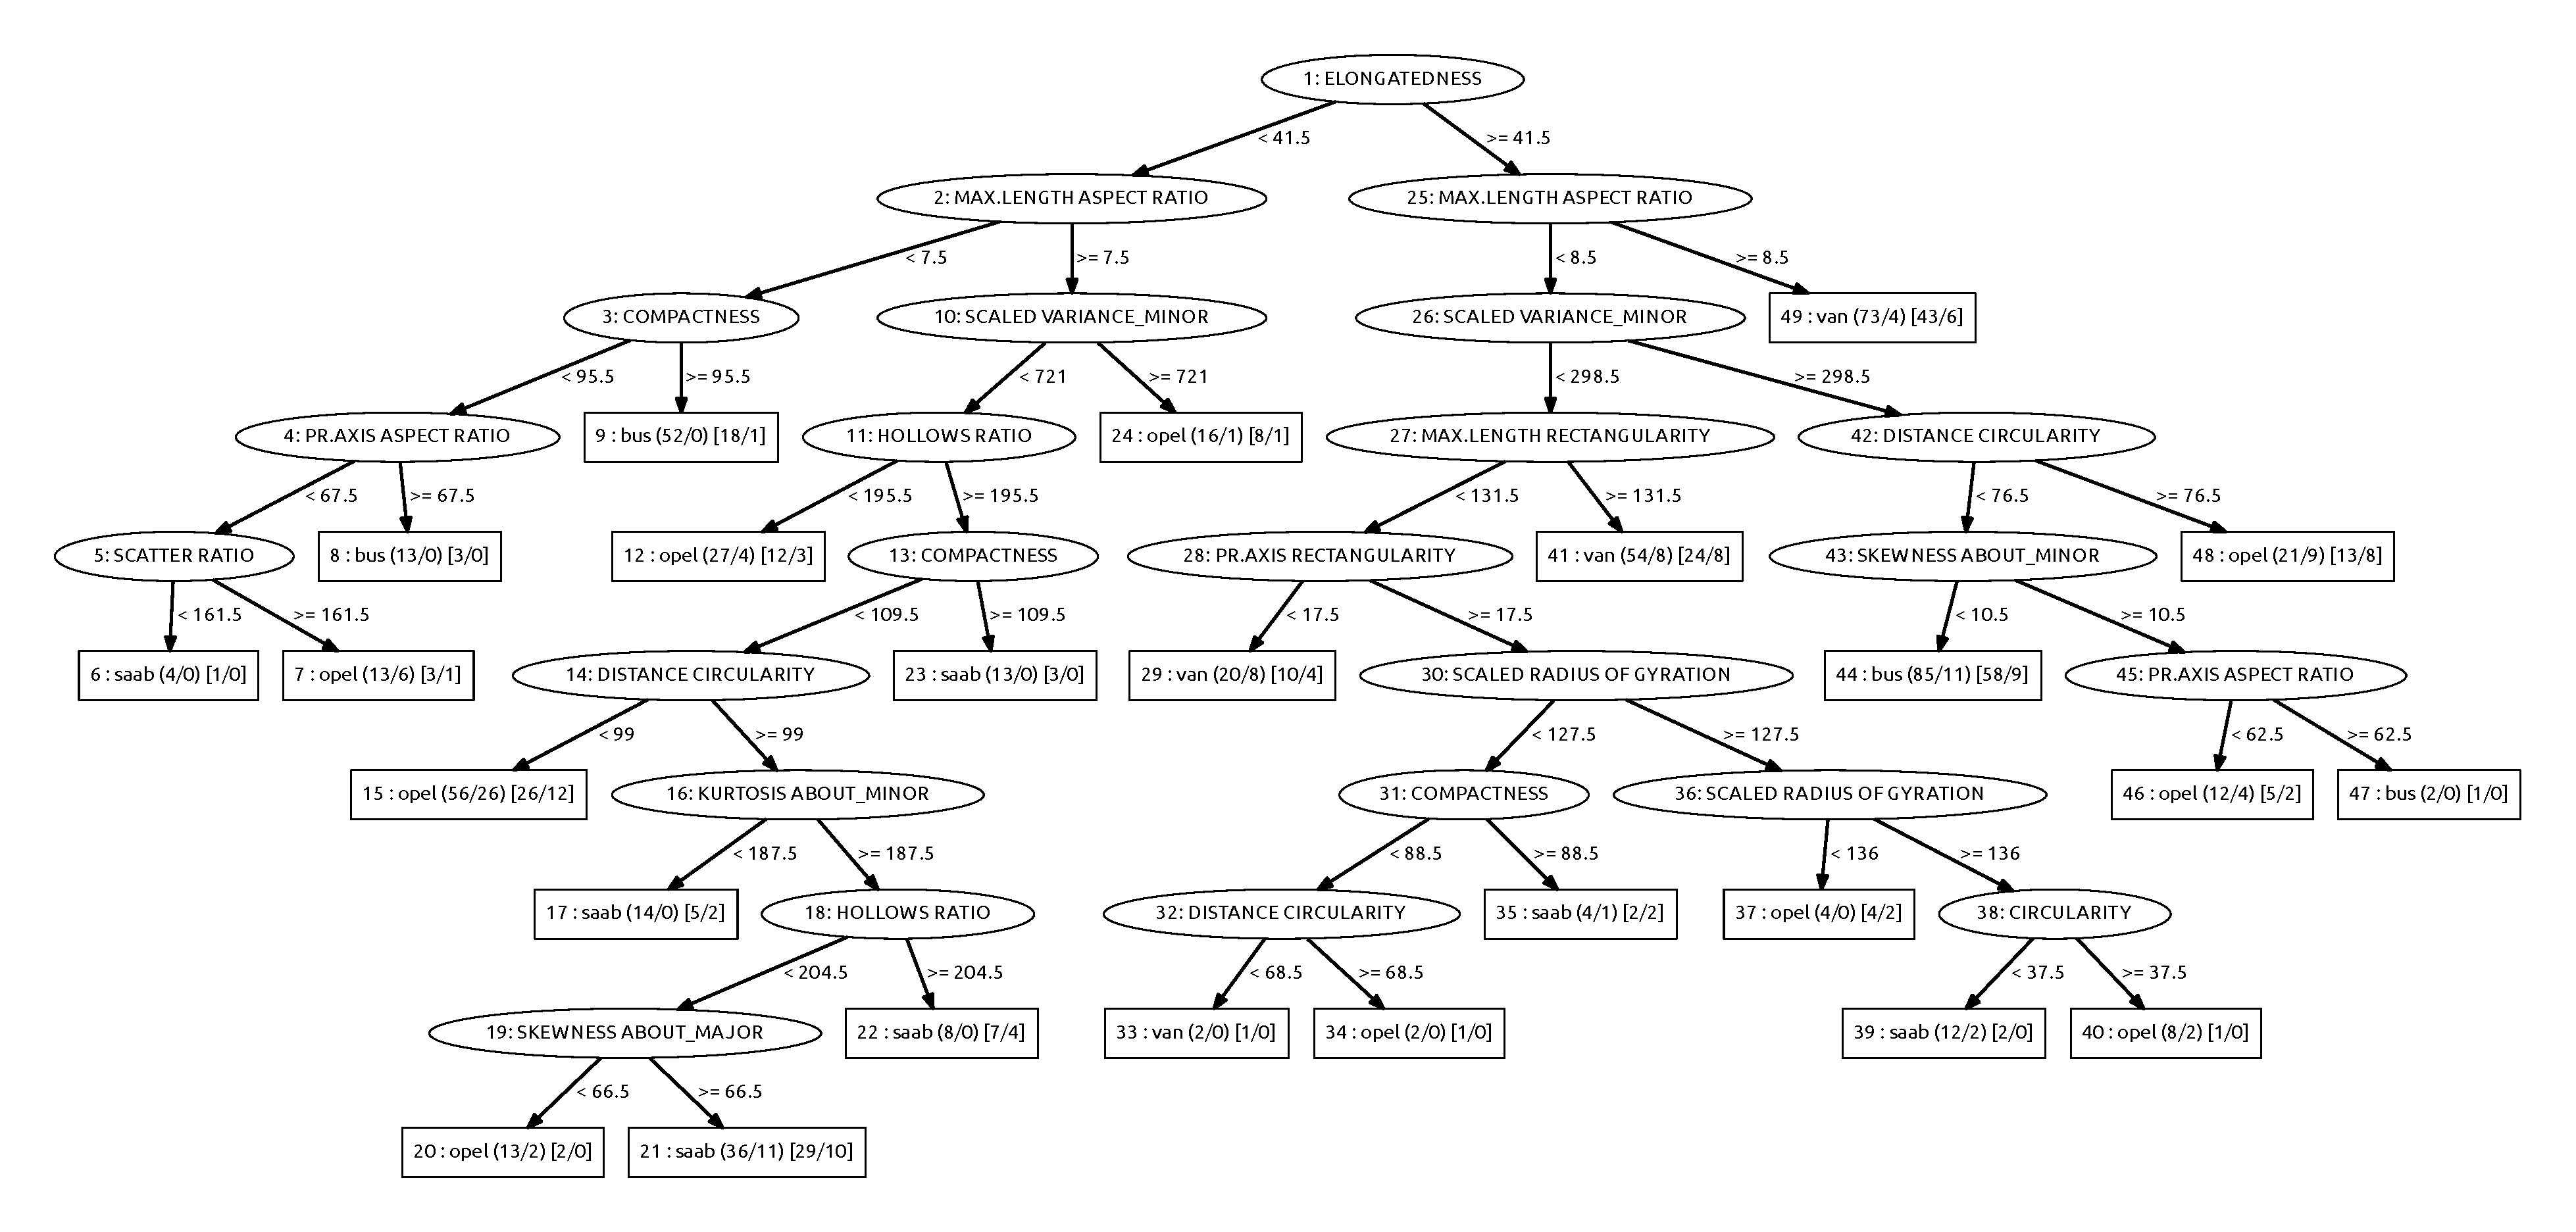
\includegraphics[width=1.55\textwidth]{results/reptree/vehicle.pdf}}
	\caption{Modello di REPTree}
\end{figure}

\begin{mdframed}[frametitle=Esecuzione JRip]
	\scriptsize\verbatiminput{results/jrip/vehicle.jrip}
\end{mdframed}


\noindent
\normalsize Regole:
\scriptsize\input{results/jrip/vehicle.list.rules}

\pagebreak

\section{Risultati su \texttt{Wisconsin Breast Cancer}}

\normalsize L'esecuzione ha coinvolto 629 istanze di training e 70 istanze di testing per ogni fold.


\begin{mdframed}[frametitle=Esecuzione NaiveBayesSimple]
	\footnotesize\verbatiminput{results/nb/wbc.nb}
\end{mdframed}


\footnotesize\input{results/nb/wbc.nbc}

\begin{mdframed}[frametitle=Esecuzione REPTree]
	\footnotesize\verbatiminput{results/reptree/wisconsin_breast_cancer.reptree}
\end{mdframed}


\begin{figure}[htb]
	\makebox[\textwidth]{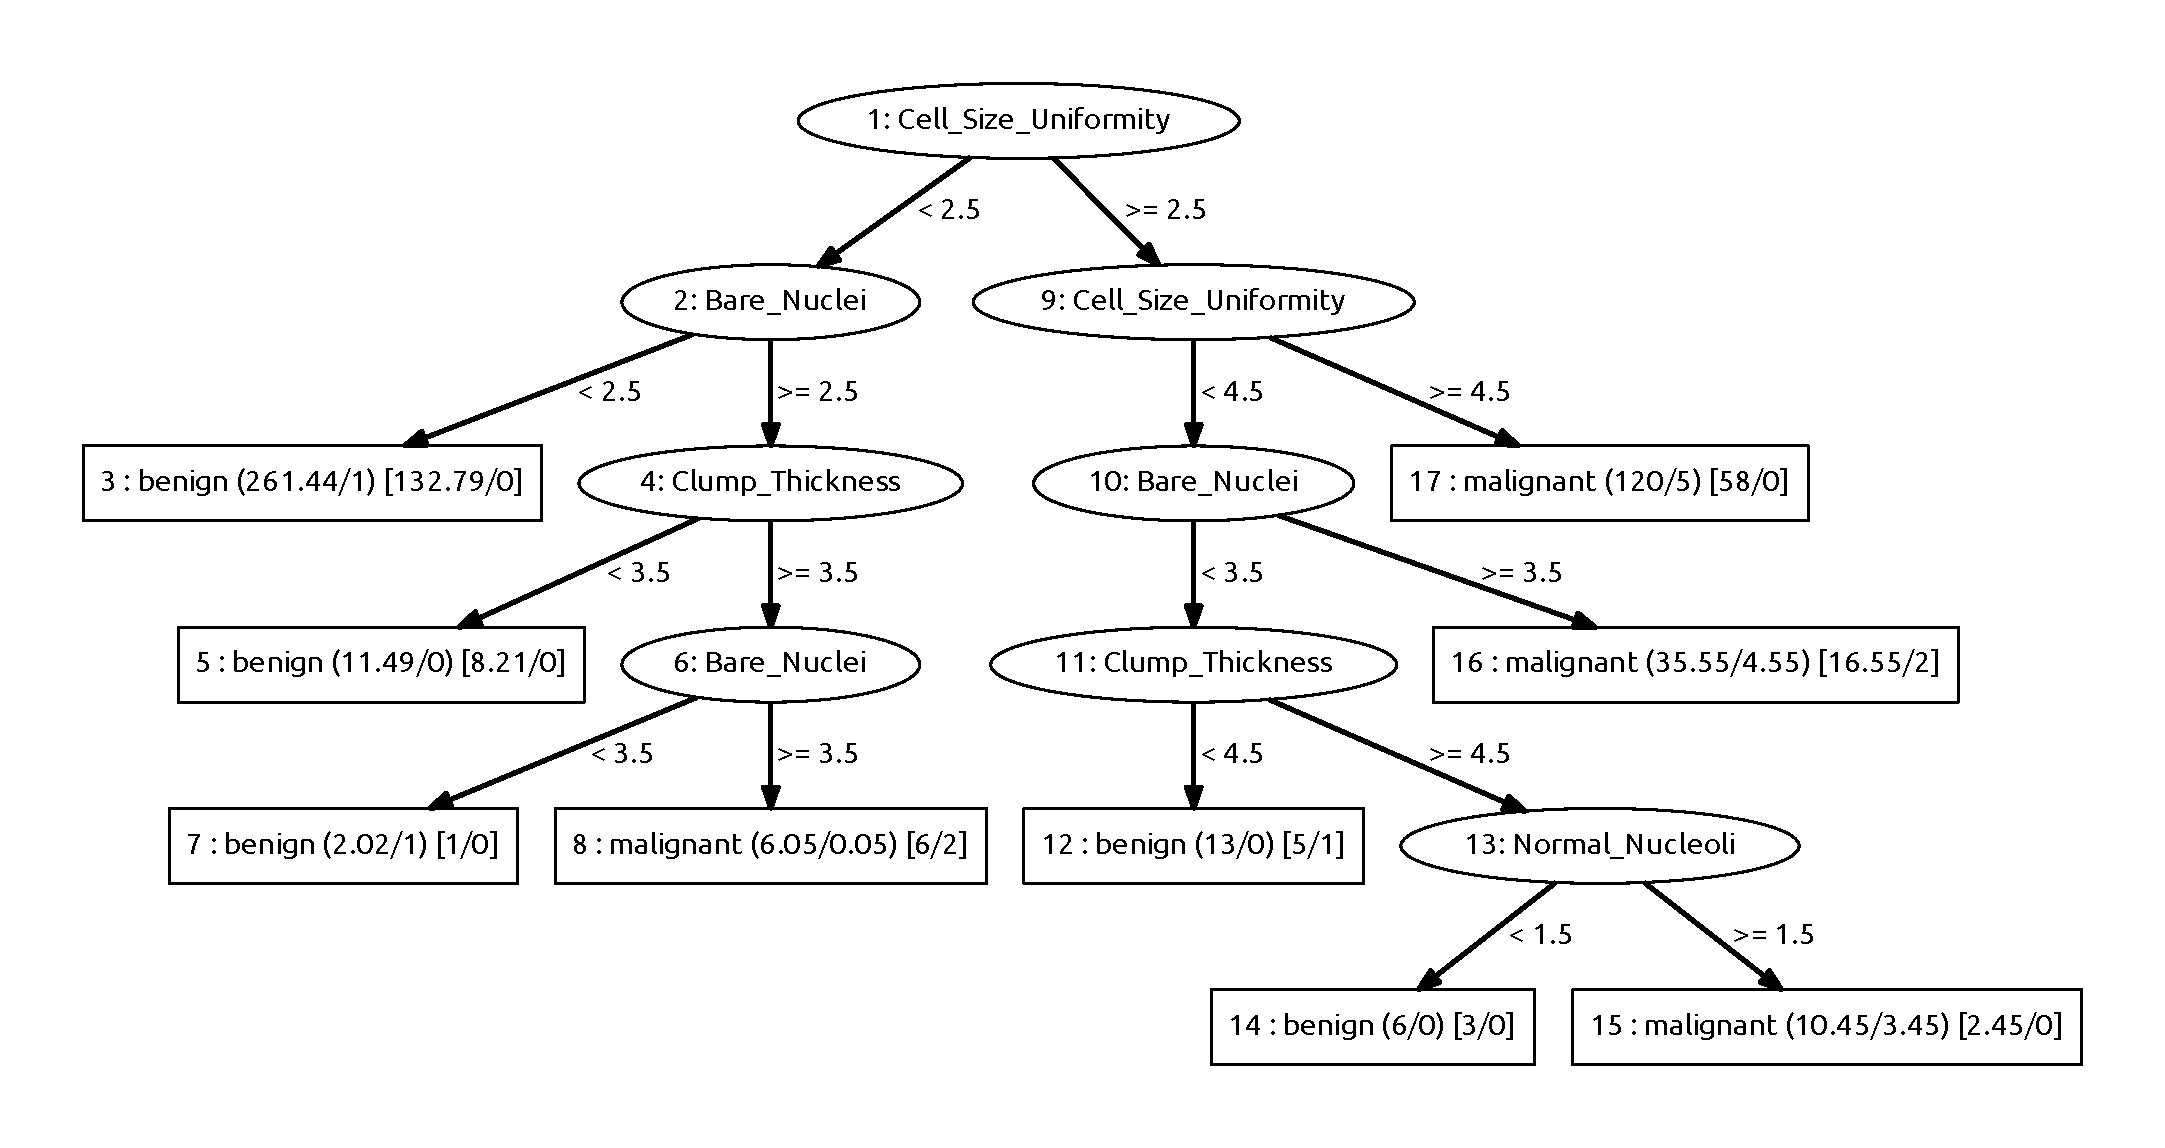
\includegraphics[width=1.55\textwidth]{results/reptree/wisconsin_breast_cancer.pdf}}
	\caption{Modello di REPTree}
\end{figure}

\begin{mdframed}[frametitle=Esecuzione JRip]
	\footnotesize\verbatiminput{results/jrip/wisconsin_breast_cancer.jrip}
\end{mdframed}


\noindent
\normalsize Regole:
\footnotesize\input{results/jrip/wisconsin_breast_cancer.list.rules}
	\clearpage
	\chapter{Analisi}

In questo capitolo verranno analizzati i risultati dell'esperimento, ottenuti utilizzando un plugin di Microsoft Excel, \textbf{XLSTAT}. La configurazione ha riguardato i valori ottenuti sui quattro dataset dai tre algoritmi di interesse: \nameref{ch:bayes}, \nameref{ch:reptree} e \nameref{ch:jrip}.

\section{Test}

Per confrontare gli algoritmi è necessario definire due ipotesi, quella nulla $H_0$ e quella alternativa $H_1$:

\begin{itemize}
	\item $H_0$: non ci sono differenze significative tra le variabili.
	\item $H_1$: almeno due variabili sono significativamente diverse tra di loro.
\end{itemize}

\noindent
Inoltre bisogna fare attenzione a scegliere lo strumento statistico adeguato, tenendo in conto alcuni aspetti:
\begin{itemize}
	\item Non possono essere fatte considerazioni sul tipo di distribuzione che i dati assumono.
	\item È necessario uno test che vada bene per più di due algoritmi.
	\item I dati non sono indipendenti tra di loro.
\end{itemize}

Per questi motivi si è scelto di utilizzare il test di \textbf{Friedman}, che è un test non-parametrico utile per gestire dati accoppiati e per funzionare con più di due algoritmi\cite{Demsar:2006:SCC:1248547.1248548}.

La metrica utilizzata è la \emph{F-Measure}, che è la media armonica di precisione e richiamo. Per fini di completezza riportiamo le relative formule:
$$Precision = \frac{True\mbox{ }Positives}{True\mbox{ }Positives + False\mbox{ }Positives}$$
$$Recall = \frac{True\mbox{ }Positives}{True\mbox{ }Positives + False\mbox{ }Negatives}$$
$$ F\mbox{-}measure = 2 \cdot \frac{Precision \cdot Recall}{Precision + Recall} $$


\subsubsection*{Esecuzione}
Di seguito vengono mostrati i dati e i risultati di esecuzione del test:

\begin{table}[!htbp]
	\centering
	\begin{tabular}{|l|r|r|r|}
		\hline
		& \multicolumn{1}{l|}{NB} & \multicolumn{1}{l|}{REPTree} & \multicolumn{1}{l|}{RIPPER} \\ \hline
		german credit & 0,748 & 0,703 & 0,697 \\ \hline
		hepatitis & 0,848 & 0,72 & 0,768 \\ \hline
		vehicle & 0,422 & 0,716 & 0,68 \\ \hline
		wisconsin bc & 0,96 & 0,939 & 0,954 \\ \hline
	\end{tabular}
	\caption{F-measure dei vari dataset}
	\label{}
\end{table}

\begin{table}[!htbp]
	\centering
	\begin{tabular}{|l|r|}
		\hline
		Valore osservato & 1,500 \\ \hline
		Valore critico & 5,991 \\ \hline
		Gradi di libertà & 2 \\ \hline
		p-value & 0,472 \\ \hline
		$\alpha$ & 0,05 \\ \hline
	\end{tabular}
	\caption{Test di Friedman}
\end{table}

\clearpage

\section{Interpretazione dei risultati}

Visto che il p-value è più grande del livello di significatività $\alpha$ = 0.05, non si può rigettare l'ipotesi nulla $H_0$, quindi gli algoritmi non si comportano diversamente gli uni dagli altri in modo statisticamente significativo.

	\clearpage
	\chapter{Conclusioni}

In questo documento sono stati confrontati tre algoritmi,  \nameref{ch:bayes}, \nameref{ch:reptree} e \nameref{ch:jrip}, su quattro dataset provienti dall'UCI Machine Learning Repository.

I risultati hanno evidenziato un pareggio tra le tre tecniche di classificazione, senza alcuna differenza significative tra di esse.

In futuro si potrebbero eseguire ulteriori test su nuovi dataset e con nuove misure per vagliare altri aspetti.
	\clearpage
	\bibliographystyle{abbrvnat}
		\bibliography{mybib}

\end{document}